%
% PCET 5.x User Manual
%
\documentclass[oneside,11pt,openany]{book}
\usepackage{amsmath}
\usepackage{graphicx}
\pagestyle{myheadings}
\markright{PCET 5.x}
\newcommand{\tw}{\ttfamily}
\makeindex

\begin{document}
%
\title{PCET User Manual}
%
\author{Alexander Soudackov\\
H\'el\`ene Decornez\\
Ivan Rostov\\
Elizabeth Hatcher\\
Christine Schwerdtfeger\\
%
\it{\small Department of Chemistry,}\\
\it{\small University of Illinois at Urbana-Champaign,}\\
\it{\small 600 S Mathews Ave,}\\
\it{\small Urbana, IL 61801}}
%
\date{Version 5.3, August 2013}

\maketitle
\frontmatter
%=======================================================================
\chapter*{About PCET}
PCET ({\bf P}roton-{\bf C}oupled {\bf E}lectron {\bf T}ransfer)
is a program package originally developed in the Sharon Hammes-Schiffer
research group at the Department of Chemistry and Biochemistry,
University of Notre Dame by A.~Soudackov, H.~Decornez and I.~Rostov in
the framework of the project "Theoretical Study of Proton-Coupled
Electron Transfer Reactions in Solution" funded by the National Science
Foundation. The package is the property of the Sharon Hammes-Schiffer
research group.

%=======================================================================
\chapter*{Disclaimer}
The developers and maintainers of the PCET package {\em do not}
guarantee that the package is free from errors. They {\em do not}
accept any responsibility for any loss or damage that may result
from its use. Users are not entitled to redistribute the program
to third parties without consent of the owners.

\tableofcontents

\mainmatter

%=======================================================================
\chapter{Introduction}
PCET is a package designed to calculate the free energy surfaces
and nonadiabatic rates of proton-coupled electron transfer reactions in
polar medium \cite{pcet-jcp1,pcet-jacs,pcet-jcp2,pcet-jpc}. The original
version combines all the original codes developed for specific model
systems and written separately by different authors. The original
main frame (A. Soudackov) included a simple ellipsoidal electrostatic
model for solvation calculations and a four-state EVB model with
standard MM parameterization for calculation of gas-phase potential.
Later this code was modified (H. Decornez) to include the Voth-Schmitt
EVB potential for water clusters. Another modification (I. Rostov)
concerned the inclusion of Frequency Resolved Cavity Model (FRCM) for
advanced solvation calculations in the framework of the dielectric continuum model.
The combined interface to all the original codes was written by A. Soudackov
and constitutes the package PCET Version 2.1. The next version 3.0
(A. Soudackov and E. Hatcher) includes additional LEPS based
two-dimensional gas-phase potentials, developed for enzyme applications,
and effects of the gating coordinate (PT donor-acceptor distance)
vibrational motion. The latest version 5.x includes modules for simulating
nonadiabatic dynamics in model PCET systems using Tully's fewest switches
surface hopping (FSSH) algorithm as well as its modifications to include
the decoherence effects. The solvent classical dynamics can be described
by the the stochastic generalized Langevin equations (GLE) of motion for the
effective solvent coordinates.

%-----------------------------------------------------------------------
\section{Functionality}

\subsection{General features}

\begin{itemize}

\item Gas-phase potentials
\begin{itemize}
\item four state EVB potentials with standard MM parameterizations
      of EVB matrix elements \cite{pcet-jacs}
\item Voth-Schmitt multistate EVB potential for water clusters
      \cite{voth-schmitt}
\item LEPS based four-state EVB potential for five-site linear
      model (enzyme applications).
\item constant potentials for modeling the electron transfer (ET)
      reactions
\end{itemize}

\item Solvent models
\begin{itemize}
\item continuum electrostatic model with ellipsoidal cavity
      \cite{Kirkwood38}
\item advanced continuum Frequency Resolved Cavity Model (FRCM)
      with cavities of molecular shape \cite{Rostov-1}
\end{itemize}

\item Free energy surfaces as functions of scalar solvent
      coordinates (on the grid or along a given path)
\begin{itemize}
\item diabatic and adiabatic free energy curves for single ET
      reaction between any two EVB states
\item adiabatic electronic/proton vibrational free energy surfaces (FES)
\item ET diabatic electronic/proton vibrational FESs
\item diabatic electronic/proton vibrational FESs
\end{itemize}

\item Rates
\begin{itemize}
\item nonadiabatic rates for single ET and PT reactions for
      any pair of EVB states
\item nonadiabatic rates as non-radiative transitions between
      two sets of ET diabatic two-dimensional free energy
      surfaces \cite{pcet-jcp2}
      \begin{itemize}
            \item averaged over gating (donor-acceptor) distances
            \item with quantum description of the gating mode
      \end{itemize}
\end{itemize}

\item Solvent mediated nonadiabatic couplings between
      adiabatic electron-proton vibrational states

\item Solvent dynamics and nonadiabatic dynamics on
      electronic (ET) and vibronic (PCET) free energy surfaces

\end{itemize}

\subsection{Quantization algorithm}
The one-dimensional Schr\"odinger equations for the proton
and gating motion are solved numerically using the Discrete
Fourier Grid Hamiltonian representation \cite{Webb-DFGH}

\subsection{Limitations}

There are two main limitations in the current version of PCET
program:
\begin{itemize}
\item the four-state MS-EVB model is implemented. It means that
      maximum two coupled charge transfer processes can be
      described. Accordingly, four different charge
      distributions in the reacting system should be defined.
\item only one quantum particle moving in one dimension
      and one gating coordinate (proton donor-acceptor distance)
      can be taken into account explicitly.
\end{itemize}

%-----------------------------------------------------------------------
\section{Programming Language}
All the routines in the current version of PCET are written
mostly in FORTRAN 90. Memory allocation is done using
FORTRAN 90 rules and syntaxis. FORTRAN 90 features
used in FRCM related routines were removed to maintain
the backward compatibility with the original FRCM code.

%-----------------------------------------------------------------------
\section{Target Computers}
Currently, PCET package can be built on the following platforms:
\begin{itemize}
\item Linux (Intel ifort and PGI pgf90 compilers with optional use of Intel MKL libraries)
\item OS X 10.7+ (GNU gfortran compiler)
\end{itemize}

%-----------------------------------------------------------------------
\section{Required External Libraries}
BLAS and LAPACK libraries (MKL libraries for Intel compiler)

%-----------------------------------------------------------------------
\section{Arithmetic Precision}
\begin{itemize}
\item All real variables and parameters are specified as {\tw real(kind=8)}
\item All integer variables are specified as {\tw integer(kind=4)}
\end{itemize}

%-----------------------------------------------------------------------
\section{Units}
The program uses kcal/mol for energy, Angstr\"oms for length, and picoseconds
for time. All the charges and masses are in atomic units.

%-----------------------------------------------------------------------
\section{The PCET directory structure}
\begin{tabular}{ll}
subdirectory & contents \\ \hline
{\tw bin}       & executable and submission scripts \\
{\tw docs}      & documentation (in TeX and PDF formats) \\
{\tw extra}     & additional codes related to the nonadiabatic rate calculations \\
{\tw source}    & FORTRAN source files, {\tw Makefile} etc. \\
{\tw tests}     & input and output files for testing \\
{\tw utilities} & analysis codes and scripts \\ \hline
\end{tabular}

%=======================================================================
\chapter{Theoretical Background}

%-----------------------------------------------------------------------
\section{Four-state Continuum Model for PCET reactions}

The electronic Hamiltonian of the PCET system (solute with
the surrounding continuum medium) is represented in the basis
of the following four valence bond (VB) states:

\begin{equation}
\begin{array}{lllcrlcrlcl}
(1a)&&\mbox{D$_{{\mathrm e}}$}^\ominus&-&^\oplus\mbox{D$_{{\mathrm p}}$}&\mbox{H}&\cdots
&\cdots&\mbox{A$_{{\mathrm p}}$}^\ominus&-&\mbox{A$_{{\mathrm e}}$} \\
(1b)&&\mbox{D$_{{\mathrm e}}$}^\ominus&-&\mbox{D$_{{\mathrm p}}$}&\cdots
&\cdots&\mbox{H}&\mbox{A$_{{\mathrm p}}$}
&-&\mbox{A$_{{\mathrm e}}$} \\
(2a)&&\mbox{D$_{{\mathrm e}}$}&-&^\oplus\mbox{D$_{{\mathrm p}}$}&\mbox{H}
&\cdots&\cdots&\mbox{A$_{{\mathrm p}}$}^\ominus&-&\mbox{A$_{{\mathrm e}}$}^\ominus \\
(2b)&&\mbox{D$_{{\mathrm e}}$}&-&\mbox{D$_{{\mathrm p}}$}&\cdots&\cdots&
\mbox{H}&\mbox{A$_{{\mathrm p}}$}&-&\mbox{A$_{{\mathrm e}}$}^\ominus.
\end{array}
\label{eq.definepcetvb}
\end{equation}
%
Here the symbols D$_{\mathrm e}$ and A$_{\mathrm e}$ represent
a general electron donor and acceptor,
D$_{\mathrm p}$ and A$_{\mathrm p}$ represent
a general proton donor and acceptor, and H represents the transferring
proton. The VB states are labeled as follows:
$a$ denotes that the proton is bonded to its donor while
$b$ denotes that the proton is
bonded to its acceptor, and
1 denotes that the electron is localized on its donor while
2 denotes that the electron is localized on its acceptor.
Thus, $a$ and $b$ indicate the proton transfer (PT) state, and
1 and 2 indicate the electron transfer (ET) state.

The electrostatic interaction of the solute with the continuum
solvent is described in terms of the two scalar solvent variables
$z_p$ and $z_e$ corresponding to the PT and ET processes,
respectively:
\begin{eqnarray}
z_p &=& \int d{\bf r}\,\,[\rho_{1b}({\bf r})-\rho_{1a}({\bf r})]
\phi_{\mathrm{in}}({\bf r}) \nonumber \\
z_e &=& \int d{\bf r}\,\,[\rho_{2a}({\bf r})-\rho_{1a}({\bf r})]
\phi_{\mathrm{in}}({\bf r}),
\end{eqnarray}
where $\rho_{ii}({\bf r})$ is the total charge density
of VB state $i$ and $\phi_{\mathrm{in}}({\bf r})$ is the inertial
polarization field of the solvent.

The electronic Hamiltonian matrix representing the free energy
of the PCET system as a function of two solute nuclear coordinates
(including the coordinate $r_p$ of the quantum particle and the gating
coordinate $R$ defined as the proton donor-acceptor distance) and
two solvent variables $z_p$ and $z_e$ has a form:
\begin{equation}
{\bf H}(r_p,R,z_p,z_e) = {\cal{S}}(r_p,R,z_p,z_e){\bf I}+ {\bf H}_o(r_p,R)
+
\left(
\begin{array}{cccc}
0&0&0&0 \\
0&z_p&0&0 \\
0&0&z_e&0 \\
0&0&0&z_p+z_e 
\end{array}
\right).
\label{eq.PCETham}
\end{equation}
The transformed self-energy ${\cal{S}}(r_p,R,z_p,z_e)$ of the solvent
inertial polarization field is expressed as
%
\begin{equation}
{\cal{S}}(r_p,R,z_p,z_e)=\frac{1}{2} \sum_{i,j=1b,2a}\bigg\{
\left[ y_{i}'+t_{1a,i}'(r_p,R)\right] \left[
{\bf t}_t'(r_p,R)^{-1}\right]_{i,j}\left[ y_{j}'+t_{1a,j}'(r_p,R)\right]
\bigg\} -\frac{1}{2} t'_{1a,1a}(r_p,R),
\end{equation}
%
where the summation runs over valence bond states $1b$ and $2a$,
the truncated reorganization energy matrix ${\bf t}_t'$ has
dimensions $2\times 2$ corresponding to these two states,
and $(z_p,z_e)\equiv (y_{1b}',y_{2a}')$. The inertial
reorganization energy matrix elements $t_{ij}'$ can
be expressed as
%
\begin{equation}
t_{ij}'=-\int d{\bf r}\,\, \nu_{jj}({\bf r})
[\hat{K}(\epsilon_o)-\hat{K}(\epsilon_\infty)]\nu_{ii}({\bf r}),
\end{equation}
%
where $\hat{K}(\epsilon)$ is the dielectric Green function
for the medium with dielectric constant $\epsilon$ and
%
\begin{eqnarray}
\nu_{1a,1a}({\bf r})&=&\rho_{1a,1a}({\bf r}) \nonumber \\
\nu_{ii}({\bf r})&=&\rho_{ii}({\bf r})-\rho_{1a,1a}({\bf r})\,\,\,\,\,
(i=1b,2a,2b).
\end{eqnarray}
%
Finally, ${\bf H}_o(r_p,R)$ is the gas phase electronic Hamiltonian
matrix.

The free energy surfaces of the system in space of the solute nuclear
coordinates and two solvent coordinates are obtained by the
diagonalization of the matrix (\ref{eq.PCETham}).

%-----------------------------------------------------------------------
\section{Mixed Electronic/Vibrational Free Energy Surfaces}
To take into account the quantum nature of the transferring proton
(or other light particle) with the coordinate $r_p$ one needs to
solve the Schr\"odinger equation
\begin{equation}
H^{\rm total}({\bf r}^{(e)},r_p,R,z_p,z_e) \Phi_n({\bf r}^{(e)},r_p;R,z_p,z_e)=
E_n(R,z_p,z_e) \Phi_n({\bf r}^{(e)},r_p;R,z_p,z_e)
\label{eq:el-vib}
\end{equation}
Here $H^{\rm total}$ is the total Hamiltonian for fixed solvent and gating
coordinates $(R,z_p,z_e)$ and can be expressed as
%
\begin{equation}
H'({\bf r}^{(e)},r_p,R,z_p,z_e)
= -\frac{\hbar^2}{2m_p}\frac{\partial^2}{\partial r_p^2} +
{\bf H}({\bf r}^{(e)},r_p,R,z_p,z_e)
\label{eq.hprime}
\end{equation}
where the first term is the kinetic energy of the transferring
proton and the second term is the electronic
Hamiltonian defined in Eq.~\ref{eq.PCETham}. The quantities
$E_n(R,z_p,z_e)$ represent the free energies of the mixed
{\em electronic/vibrational} (vibronic) states
$\Phi_n({\bf r}^{(e)},r_p;R,z_p,z_e)$.

In the case of the quantization along the gating coordinate...

\subsection{Methods of Solution of Eq.(\ref{eq:el-vib})}

In the program PCET, three different methods of solution
of the equation (\ref{eq:el-vib}) are implemented. In
all these methods the total Hamiltonian is represented
in the basis of the products of electronic and vibrational
wavefunctions.

\subsubsection{Method 1: based on diabatic electronic states}
In this approach the mixed electronic/proton
vibrational adiabatic states are expanded in a basis of
products of diabatic electronic states and corresponding
adiabatic proton vibrational states. The approach consists
of three steps.

The first step is to
calculate the energies of the electronic diabatic states for fixed
solvent coordinates $(z_p,z_e)$ 
for all points $r_p$ along a one-dimensional grid
between the proton donor and acceptor.  The energy of the diabatic
electronic state $i$ is 
%
\begin{equation}
E_i^{\mathrm{(dia)}}(r_p,z_p,z_e)=H_{ii}(r_p,z_p,z_e)
\end{equation}
\par
The second step is to calculate the proton vibrational
adiabatic states $\phi_\mu^{(i)}(r_p;z_p,z_e)$ for
fixed solvent coordinates for each diabatic electronic state $i$
by numerically solving the one-dimensional Schr\"odinger equation
%
\begin{equation}
\left( -\frac{\hbar^2}{2m_p}\frac{\partial^2}{\partial r_p^2}
+E_i^{\mathrm{(dia)}}\right)
\phi_\mu^{(i)}(r_p;z_p,z_e)=\epsilon_\mu^{(i)}(z_p,z_e)
\phi_\mu^{(i)}(r_p;z_p,z_e).
\end{equation}
%
This equation is solved
by expanding the proton vibrational states 
on a grid along the axis between the
proton donor and acceptor and implementing standard discrete
Fourier grid techniques.
\par
The third step in this approach is to calculate the 
numerically exact mixed electronic/proton
vibrational adiabatic states by expanding them in terms of
basis states each comprised of a product of an electronic diabatic state $i$
and a proton vibrational adiabatic state $\phi_\mu^{(i)}$.
The mixed electronic/vibrational states are calculated by
solving the matrix equation
%
\begin{equation}
{\bf H}^{\rm total} {\bf D}={\bf D}{\bf E},
\end{equation}
%
where ${\bf D}$ has elements $D_{i\mu,n}$, ${\bf E}$ is diagonal with
elements $E_{n}$, and
the matrix elements of the Hamiltonian ${\bf H}^{\rm total}$ are
%
\begin{equation}
H_{i\mu,j\nu}^{\rm total} =
\delta_{ij}\delta_{\mu\nu}\epsilon_\mu^{(i)}(z_p,z_e)+
(1-\delta_{ij})\left\langle \phi_\mu^{(i)}\left|
{H}_{ij}\right|\phi_\nu^{(j)}\right\rangle_p .
\label{eq.hinjmd}
\end{equation}
%
(Here $\langle \ldots \rangle_p$ indicates integration over $r_p$.)
The energies of the mixed electronic/proton vibrational
adiabatic states can be calculated
as functions of the two solvent scalar variables $z_p$ and $z_e$
by following these three steps for solvent coordinates $(z_p,z_e)$
on a two-dimensional grid.

\subsubsection{Method 2: based on adiabatic electronic states}
In this approach the mixed electronic/proton
vibrational adiabatic states are expanded in a basis of
double adiabatic states. The approach consists of three steps.
The first step is to calculate the electronic
adiabatic states $\Psi_k({\bf r}^{(e)};r_p,z_p,z_e)$ 
for fixed solvent
coordinates $(z_p,z_e)$ for all points $r_p$ along a one-dimensional grid
between the proton donor and acceptor.
The electronic wavefunction
$\Psi_k$ is a linear combination of
the four valence bond states (1a, 1b, 2a, 2b).
The energy of electronic state $k$ is
${\cal U}_k(r_p,z_p,z_e)$ obtained by diagonalizing
the matrix ${\bf H}$ defined in Eq.~\ref{eq.PCETham}.
\par
The second step of this prescription is to calculate the proton
vibrational adiabatic states $\phi_\mu^{(k)}(r_p;z_p,z_e)$
for fixed $(z_p,z_e)$
for each relevant adiabatic electronic state $k$ by numerically solving
the one-dimensional Schr\"odinger equation
\begin{equation}
H_p^{(k)} \phi_{\mu}^{(k)}(r_p;z_p,z_e)=
\epsilon_{\mu}^{(k)}(z_p,z_e) \phi_\mu^{(k)}(r_p;z_p,z_e),
\label{eq.pcetpts}
\end{equation}
where the proton Hamiltonian for the electronic state $k$ is defined as
\begin{equation}
H_p^{(k)}=-\frac{\hbar^2}{2m_p}\frac{\partial^2}{\partial r_p^2}
+{\cal U}_k(r_p,z_p,z_e).
\label{eq.protham}
\end{equation}
\par
The third step of the prescription is
to calculate the
mixed electronic/proton vibrational adiabatic states $\Phi_n$ by expanding them
in a basis of double adiabatic states $\xi_{k\mu }$:
\begin{equation}
\Phi_n({\bf r}^{(e)},r_p;z_p,z_e)=\sum_{k\mu} 
D_{k\mu,n} \xi_{k\mu}({\bf r}^{(e)},r_p;z_p,z_e)
\end{equation}
where
\begin{equation}
\xi_{k\mu}({\bf r}^{(e)},r_p;z_p,z_e)
=\Psi_k({\bf r}^{(e)};r_p,z_p,z_e) \phi_\mu^{(k)}(r_p;z_p,z_e).
\label{basisfunc}
\end{equation}
The mixed electronic/vibrational states are calculated by
solving the matrix equation
\begin{equation}
{\bf H}^{\rm total} {\bf D}={\bf D}{\bf E},
\end{equation}
where ${\bf D}$ has elements $D_{k\mu,n}$, ${\bf E}$ is diagonal with
elements $E_{n}$, and
the matrix elements of the Hamiltonian ${\bf H}^{\rm total}$ are
\begin{equation}
H_{k\mu,l\nu}^{\rm total} = \langle \xi_{k\mu}|H^{\rm total}|\xi_{l\nu}\rangle.
\end{equation}
It is straightforward to show that
\begin{equation}
H_{k\mu,l\nu}^{\rm total} =
\delta_{kl}\delta_{\mu\nu}\epsilon_\mu^{(k)}(z_p,z_e)
- \frac{\hbar^2}{m_p}\left\langle \phi_\mu^{(k)}\left|
d_{kl}^{(ep)} \frac{\partial \phi_\nu^{(l)}}{\partial r_p} 
\right.\right\rangle_p
- \frac{\hbar^2}{2m_p}\langle \phi_\mu^{(k)}|
g_{kl}^{(ep)}\phi_\nu^{(l)} \rangle_p,
\label{eq.hinjm}
\end{equation}
where
\begin{equation}
d_{kl}^{(ep)}(r_p,z_p,z_e)
=\left\langle \Psi_k \left| \frac{\partial \Psi_l}{\partial r_p} 
\right.\right\rangle_e
\label{epnonad1}
\end{equation}
and
\begin{equation}
g_{kl}^{(ep)}=\left\langle \Psi_k\left|\frac{\partial^2 \Psi_l}{\partial r_p^2}
\right.\right\rangle_e.
\label{epnonad2}
\end{equation} 
In these
equations $\langle \rangle_{ep}$, $\langle \rangle_e$, and $\langle \rangle_p$
indicate integration over $({\bf r}^{(e)}, r_p)$, ${\bf r}^{(e)}$, and
$r_p$, respectively.
\par
The energies of the mixed electronic/proton vibrational
adiabatic states are calculated
as functions of the two solvent scalar variables $z_p$ and $z_e$
by following the above three steps for solvent coordinates $(z_p,z_e)$
on a two-dimensional grid.

\subsubsection{Method 3: double-adiabatic approach}
This method is actually an approximation to the method 2
described above. It is assumed that the nonadiabatic coupling
terms $d_{kl}$ and $g_{kl}$ defined in Eqs.(\ref{epnonad1})
and (\ref{epnonad2}) are negligibly small and the total Hamiltonian
matrix is diagonal in the double adiabatic representation.
Thus the free energies are equal to the double-adiabatic
energies $\epsilon_\mu^{(k)}(z_p,z_e)$.

\subsection{Free Energy Surfaces in Different Representations}
In some specific cases it is useful to analyze different
types of free energy electronic/vibrational surfaces.
The program PCET can calculate free energies in three different
representations.

\subsubsection{Adiabatic Free Energy Surfaces ({\tw ADIAB})}
This is a most general representation. The corresponding states
are {\em adiabatic} with respect to the solvent motions and
all the couplings between the electronic EVB states as well
as all the nonadiabatic couplings between electronic and
proton motions are taken into account explicitly. The free
energies are calculated as eigenvalues of the total Hamiltonian
$H^{\rm total}$.

\subsubsection{ET-Diabatic Free Energy Surfaces ({\tw DIAB2})}
This representation is natural for the systems with strongly
nonadiabatic ET and adiabatic PT when the couplings between (1a/1b)
and (2a/2b) electronic VB states are small compared to the thermal energy
$k_{\rm B}T$. The two sets of the corresponding free energies
and mixed electronic/vibrational ET diabatic states are obtained
by applying one of the above mentioned methods to (1a/1b) or
(2a/2b) blocks of the electronic Hamiltonian matrix (\ref{eq.PCETham}).

\subsubsection{Diabatic Free Energy Surfaces ({\tw DIAB4})}
This representation is natural for the systems with strongly
nonadiabatic ET and PT when all the couplings between electronic
VB states are small compared to the thermal energy $k_{\rm B}T$.
Formally, it corresponds to the electronic Hamiltonian matrix
(\ref{eq.PCETham}) with zero off-diagonal matrix elements.

%-----------------------------------------------------------------------
\section{Gas Phase Model Potentials}
The model gas phase potentials implemented in the program are
based on the four-state EVB model with electronic basis states
defined in Eq.(\ref{eq.definepcetvb}). They differ by the
parameterization of the EVB matrix elements.

\subsection{Standard MM parameterization ({\tw MM1})}
The matrix elements of the gas phase Hamiltonian are approximated
by standard molecular mechanical terms fit to electronic structure
calculations for the gas phase solute. The diagonal matrix
elements are expressed as
%
\begin{eqnarray}
(h_{0})_{1a1a}(r_p) &=& U^{\rm{Morse}}_{NH}(r_p) + U^{\rm{rep}}_{OH}(r_p) +
U^{\rm{Coul}}_{1a}(r_p) \\ \nonumber
(h_{0})_{1b1b}(r_p) &=& U^{\rm{Morse}}_{OH}(r_p) + U^{\rm{rep}}_{NH}(r_p) +
U^{\rm{Coul}}_{1b}(r_p) + \Delta_{1b}\\ \nonumber
(h_{0})_{2a2a}(r_p) &=& U^{\rm{Morse}}_{NH}(r_p) + U^{\rm{rep}}_{OH}(r_p) +
U^{\rm{Coul}}_{2a}(r_p) + \Delta_{2a}\\ \nonumber
(h_{0})_{2b2b}(r_p) &=& U^{\rm{Morse}}_{OH}(r_p) + U^{\rm{rep}}_{NH}(r_p) +
U^{\rm{Coul}}_{2b}(r_p) + \Delta_{2b}
\label{eq.MM}
\end{eqnarray}
%
where
%
\begin{equation}
U^{\rm{Morse}}_{AH}(r_p) = D_{AH}\left(1-e^{-\beta_{AH}(R_{AH}-R_{AH}^{o})}\right)^2
\label{Morse}
\end{equation}
%
is a Morse potential for an A-H bond,
%
\begin{equation}
U^{\rm{rep}}_{AH}(r_p) = D'_{AH}e^{-\beta'_{AH}R_{AH}}
\label{Rep}
\end{equation}
%
is a repulsion term between non-bonded atoms A and H, and
%
\begin{equation}
U^{\rm{Coul}}_{i}(r_p) = \frac{1}{2}\sum_{k\ne l}\frac{q_k^{i}q_l^{i}}{R_{kl}}
\label{Coul}
\end{equation}
%
is a Coulomb interaction potential between the point charges 
(where the summation is over
sites $k,l$ and $q_k^i$ is the charge on site $k$ for VB state $i$).
In all of these expressions $R_{kl}$ is the distance between sites
$k$ and $l$.
%
The couplings between the VB states are expressed as
%
\begin{eqnarray}
(h_o)_{1a,1b}(r_p) &=&  V^{PT1}\exp^{-\gamma_{\rm PT}(r_p-r_p^{\rm PT})^2}\\ \nonumber
(h_o)_{2a,2b}(r_p) &=&  V^{PT2}\exp^{-\gamma_{\rm PT}(r_p-r_p^{\rm PT})^2}\\ \nonumber
(h_o)_{1a,2a}(r_p) &=& (h_o)_{1b,2b}(r_p)
 = V^{ET}\exp^{-\gamma_{\rm ET}(r_p-r_p^{\rm ET})^2}  \\ \nonumber
(h_o)_{1a,2b}(r_p) &=& (h_o)_{1b,2a}(r_p)
 = V^{EPT}\exp^{-\gamma_{\rm EPT}(r_p-r_p^{\rm EPT})^2}.
\label{eq.offdiagparam}
\end{eqnarray}
%

\subsection{Two-dimensional LEPS potential}

\subsection{Voth-Schmitt parameterization for water clusters}






%-----------------------------------------------------------------------
\section{Solvation models}
\subsection{Ellipsoidal Model}
In this model the solute is represented by a set of point charges
located on one axis. Different charge distributions corresponding
to VB basis states are modelled by different magnitudes of point
charges. The point charges representing the solute are placed
on the main axis of an axially symmetrical ellipsoidal cavity
embedded in a dielectric continuum solvent characterized by the
inertial ($\epsilon_0$) and electronic (optical) ($\epsilon_\infty$)
dielectric constants (see Fig.~\ref{fig1}).
\begin{figure}[!bbb]
\begin{center}
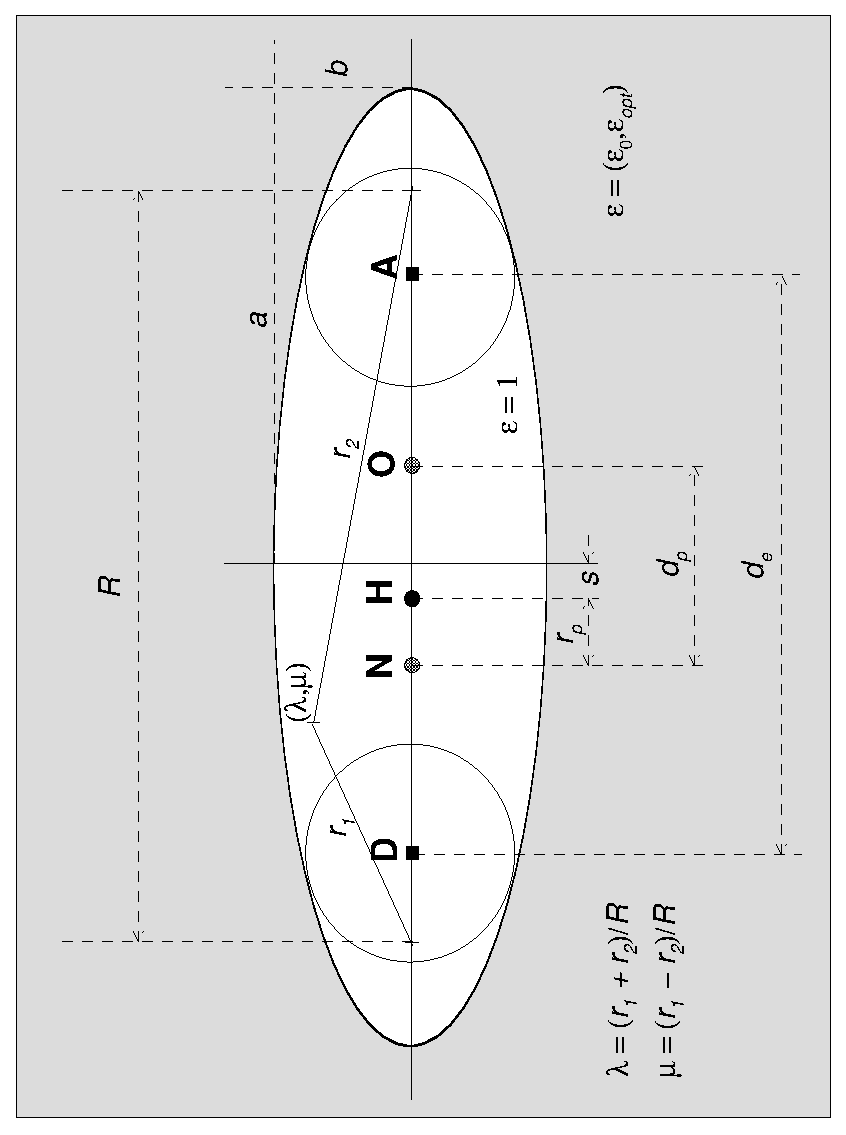
\includegraphics[scale=0.65,angle=-90]{ellips.eps}
\end{center}
\caption{Ellipsoidal model cavity and its geometrical parameters.}
\label{fig1}
\end{figure}
\par
The total polarization potential $\phi(\mu,\lambda)$ at the point ($\mu$,$\lambda$) (elliptical coordinates) inside the cavity
can be expressed as\cite{Kirkwood38}
\begin{equation}
\phi(\mu,\lambda)=\sum_{n=0}^{\infty}B_n(\epsilon_0)P_n(\mu)P_n(\lambda)
\label{phi_tot}
\end{equation}
where $B_n$ are constants and $P_n$ are the Legendre functions
of the first kind. The expression for the coefficients $B_n$
is readily obtained from traditional electrostatics:
\begin{equation}
B_n=\frac{2(2n+1)\beta_n}{R}\left(\frac{1}{\epsilon_0}-1\right)
\frac{Q_n(\lambda_0)}{P_n(\lambda_0)}
\left[1-\frac{1}{\epsilon_0}
\frac{\lambda_0-P_{n-1}(\lambda_0)/P_n(\lambda_0)}
     {\lambda_0-Q_{n-1}(\lambda_0)/Q_n(\lambda_0)}
\right]^{-1}
\label{bcoef}
\end{equation}
Here $R$ is the interfocal distance, $\lambda_0$ defines the
ellipsoid boundary, $Q_n$ are the Legendre functions of the
second kind, and $\beta_n$ is given by the sum over the N
point charges with magnitudes $q_k$ and positions on the axis
$\mu_k$
\begin{equation}
\beta_n=\sum_{k=1}^N q_kP_n(\mu_k)
\label{beta}
\end{equation}
\par
The inertial polarization field is calculated as a difference
between the total field and the electronic polarization field:
\begin{equation}
\phi_{\mathrm in} = \phi - \phi_{\infty}
\label{phi_in}
\end{equation}
where $\phi_{\infty}$ is obtained using
Eqs.(\ref{phi_tot}-\ref{bcoef}) by substituting $\epsilon_0$
in Eq.(\ref{bcoef}) with $\epsilon_{\infty}$.
\par
The reorganization energy matrix elements are calculated
then on the grid along the proton coordinate by using standard definitions\cite{pcet-jcp1}:
\begin{eqnarray}
t_{ij} &=& -\sum_k q_k^{(i)}(\phi^{(j)}-\phi^{(j)}_{\infty}) \\
t_{ij}^{(\infty)} &=& -\sum_k q_k^{(i)}\phi^{(j)}_{\infty}
\label{tmat}
\end{eqnarray}
where indices $i$ and $j$ label charge distributions corresponding
to the VB basis states.


\subsection{FRCM}

Relevant references:
\begin{itemize}
\item{Chudinov, Napolov, and Basilevsky, Chemical Physics {\bf 160}, 41-54 (1992).}
\item{
Basilevsky, Rostov, and Newton, Chemical Physics {\bf 232}, 189-199 (1998).}
\item{
Soudackov and Hammes-Schiffer, J. Chem. Phys. {\bf 111}, 4672 (1999).}
\end{itemize}
\section*{Description of algorithm}
\subsection*{Reorganization energy matrix elements}
The multistate continuum theory requires the calculation
of the solvent
reorganization energy matrix elements defined as
\begin{equation}
t_{ij}=-\int d{\bf r}\, \rho_i \hat{\cal{K}}_{\mathrm{in}} \rho_j
= -\int d{\bf r}\, \rho_i \phi_j^{\mathrm{(in)}},\,\,\, \phi_j^{\mathrm{(in)}}=\hat{\cal{K}}_{\mathrm{in}} \rho_j
\end{equation}
and
\begin{equation}
t_{ij}^{(\infty)}=-\int d{\bf r}\, \rho_i \hat{\cal{K}}_{\infty} \rho_j
= -\int d{\bf r}\, \rho_i \phi_j^{(\infty)},\,\,\, \phi_j^{(\infty)}=\hat{\cal{K}}_{\infty} \rho_j.
\end{equation}
Here the operator $\hat{\cal{K}}_\infty=\hat{\cal{K}}(\epsilon_\infty)$
and $\hat{\cal{K}}_{\mathrm{in}}=\hat{\cal{K}}(\epsilon_o)-
\hat{\cal{K}}(\epsilon_\infty)$,
where $\hat{\cal{K}}(\epsilon)$ is a dielectric Green
function for the medium with dielectric constant $\epsilon$ and
$\epsilon_o$ and $\epsilon_\infty$ are the static and
electronic dielectric constants, respectively.
The calculation of these reorganization energies
requires the calculation of the potentials
$\phi_j^{(\infty)}=\hat{\cal{K}}(\epsilon_\infty) \rho_j$ and
$\phi_j^{\mathrm{(tot)}} = \hat{\cal{K}}(\epsilon_o) \rho_j$
caused by the charge density $\rho_j$ in a dielectric continuum
with dielectric constant $\epsilon_\infty$ and $\epsilon_o$, respectively.
The inertial potential may be calculated from these
two potentials: 
\begin{equation}
\phi_j^{\mathrm{(in)}}=\phi_j^{\mathrm{(tot)}}
- \phi_j^{\mathrm{(\infty)}}.
\label{eq.phiin}
\end{equation}
The FRCM method is used to calculate these potentials.
%
\subsection*{Calculation of the electrostatic potential due to solvent response}
%
The standard PCM method is used to calculate the
electronic solvent potential $\phi_j^{(\infty)}$.
In this method,
the entire charge density $\rho_j$ is placed in a
cavity of arbitrary shape with surface $S$.
The dielectric
constant is equal to unity
inside the cavity and is equal to $\epsilon_\infty$
outside the cavity.
The electronic solvent potential $\phi_j^{(\infty)}$ is calculated by solving
the Poisson equation
with the appropriate boundary conditions at the surface of the
cavity.
(Note that the total potential used in the Poisson
equation is the sum of the potential
due to the charge density $\rho_j$ in a vacuum
and the solvent potential $\phi_j^{(\infty)}$ describing 
the potential due to the solvent response to the density $\rho_j$.)
The solvent potential 
may be expressed in terms of a surface charge density $\sigma_j$
on the surface $S$.  Thus, the problem is reduced to
the calculation of
this surface charge density $\sigma_j$ corresponding
to the charge density $\rho_j$.
The surface charge density $\sigma_j$ may be defined
in terms of a standard integral equation, which must
be solved iteratively.  
\par
The FRCM method is used to calculate the
total solvent potential $\phi_i^{\mathrm{(tot)}}$.
In this method,
two cavities are formed around the charge density $\rho_j$.  
This leads to an inner
surface $S_1$ and an outer surface $S_2$.
The entire charge density is assumed to be
contained inside the inner cavity.
The dielectric constant is equal to unity inside
the inner cavity, to $\epsilon_\infty$ in the
region between the two surfaces $S_1$ and $S_2$, and to $\epsilon_o$
in the region outside the outer cavity.
The solvent potential $\phi_j^{\mathrm{(tot)}}$ is calculated by solving
the Poisson equation
with the appropriate boundary conditions at the two surfaces
$S_1$ and $S_2$.
(Again, note that the total potential used in the Poisson
equation is the sum of the potential
due to the charge density $\rho_j$ in a vacuum
and the solvent potential $\phi_j^{\mathrm{(tot)}}$ describing 
the potential due to the solvent response to the density $\rho_j$.)
The solvent potential 
may be expressed in terms of two surface charge distributions
$\sigma_j^{(1)}$ and $\sigma_j^{(2)}$ on the surfaces $S_1$ and $S_2$, 
respectively.
In this case, the problem requires
the calculation of
both surface charge distributions corresponding
to the charge density $\rho_j$.
These surface charge densities may be defined
in terms of integral equations which must
be solved iteratively.  
\par
In order to numerically solve
the integral equations for both PCM and FRCM, the
surface integrals are computed
by dividing the surface into small pieces.  
These surface
elements are denoted ``tesserae" or  ``sectors" (where the terms
are used interchangably, although a
sector actually refers to a three-dimensional segmenet
and a tesserae actually refers to only the surface element).
The convergence of the iterative solution of the Poisson equation is
determined by the dimensionless parameter SELFCR, where
the convergence criterion is defined to be SELFCR$\times 10^{-4}$
for the outer cavity and SELFCR$\times 10^{-5}$ for the inner cavity.
The default is SELFCR=2.0.  In past versions, the keyword PRECISE 
decreases this to SELFCR=0.2, but
this word should not be used in the current version.
After the surface charge density has converged, it is
renormalized according to the total charge of the solute.
If the total surface charge computed from the
numerical surface charge density differs from the value
determined by the total solute charge
by more than CHDIFF directly prior to the renormalization
of the surface charge density, an error message
is printed.  The default value
is CHDIFF=0.1.
The maximum number of iterations is ITSE, after which an
error message is printed and the program is stopped.
The default value is ITSE=15.
\par
Thus, the calculation of the electronic and inertial
potentials requires the following steps:
\begin{enumerate}
\item{Generate the surfaces of the two cavities.}
\item{Generate the tesserae independently for the two cavities.}
\item{Numerically solve the Poisson equation using PCM for the inner
cavity surrounded by solvent with dielectric constant $\epsilon_\infty$
to obtain the electronic potential $\phi_j^{(\infty)}$.}
\item{Numerically solve the Poisson equation using FRCM for the two cavities
with solvent of dielectric constant $\epsilon_\infty$ in between
the two surfaces and $\epsilon_o$ outside both cavities
to obtain the total potential $\phi_j^{\mathrm{(tot)}}$.}
\item{Calculate the inertial
potential $\phi_j^{\mathrm{(in)}}=\phi_j^{\mathrm{(tot)}}
- \phi_j^{(\infty)}$.}
\item{Use these potentials to calculate the electronic
and inertial reorganization energy matrix elements.}
\end{enumerate}
%
\subsection*{Generation of surfaces}
%
In FRCM, the inner cavity is generated by placing
a sphere centered on each atom with radius $\kappa r_{vdw}$,
where $r_{vdw}$ is the van der Waals radius for the specific atom
and $\kappa$ is independent of the solvent
with a default value of 0.9.
In the FRCM program, the surface of the inner cavity
may be smoothed by including additional spheres.
The key words SMOOTH and NOSMOOTH denote cavity smoothing
or the absence of cavity smoothing.  The default is to include
smoothing.  
The parameter SOLRD defines the effective radius (in Angstroms) of the solvent
molecules and is used to calculate the excluded volume at the
seam of a pair of overlapping spheres.
The default value is SOLRD=1~\AA.
The parameter EXVOL defines
the minimum excluded volume (in cubic Angstroms) at such a seam
for which an auxiliary sphere is
added during smoothing.  The default value is EXVOL=1~\AA$^{3}$.
If EXVOL (or SOLRD) is large enough, the effect is the same as
using the key word NOSMOOTH.
The outer sphere cavity is generated by adding
$\delta$ to the radius of each sphere used to create
the inner cavity (including the spheres added for smoothing).
In general, $\delta$ depends on the solvent.
%
\subsection*{Generation of tesserae/sectors}
%
The premise of the method for generation of the tesserae (or sectors)
is that the surface charges
change more rapidly closer to the seam of the intersection
between two spheres.  Thus, the surface elements should be
chosen to be smaller in the regions of close contact of the spheres.
The following three steps are used to generate the tesserae.
\begin{enumerate}
\item{The first step
is to create a network of A-sectors for each pair of spheres.  
These sectors
are smaller in contact regions (i.e., where the spheres overlap) and larger
in regions near the poles.
The tesserae are created through a series
of rings moving from a contact region to a pole.
The tesserae (or sectors) are defined in terms of
the standard polar angles $\theta$ and $\phi$, where
$0<\theta<180^o$ and $0<\phi<360^o$, and $\theta$
is measured relative to the axis connecting the centers of the pair
of spheres.  The parameters that determine the sizes of the A-sectors
and the basic procedure used to create the A-sectors
are as follows.
\begin{itemize}
\item{The parameters that determine the sizes of the A-sectors
are MODFE1 and MODFE2 for the inner and outer surfaces,
respectively.  
This discussion will use MODFE1 as the example.
The maximum angular step size $\Delta \theta$ for $\theta$ is defined
as 
\begin{equation}
N=400/3/\mbox{MODFE1}.
\end{equation}
For the default value of MODFE1=6, $N=22.2^o$.
The first two rings near the contact region have
$\Delta \theta=0.6N$ and $\Delta \theta =0.9N$, respectively, and the remaining
rings have $\Delta \theta= N$.
The values for these angular step sizes are stored in the
array DDTET, where the first element is $0.6N$,
the second element is $0.9N$, and the remaining elements are $N$.
The number of elements is such that the sum of all angles
is less than 180$^o$.  Thus, for MODFE1=6,
DDTET=(13.3, 20.0, 22.2, 22.2, 22.2, 22.2, 22.2, 22.2).
The angle $\phi$ has the same angular step size $\Delta \phi$ as $\theta$
except for the first two rings, where $\Delta \phi=1.33 \Delta \theta$
and $\Delta \phi=1.28 \Delta \theta$, respectively.}
\item{
The A-sectors are created for each pair in the following manner.
First, the angle in $\theta$ for the overlap between the spheres
is determined to exclude it from consideration.
Second, the sectors are created through a series of rings, using
the angular step sizes from the array DDTET,
starting at the contact
region and moving toward the pole.
The sectors are renormalized to render the total sum of
angular steps
for $\theta$ and $\phi$ $180^o$ and $360^o$, respectively.
Since this procedure is done for each pair of spheres,
for each sphere there is a combination of overlapping
networks of A-sectors due to all of its neighbors.}
\item{
The relation between MODFE1 and MODFE2 is critical to the numerical
accuracy.  Typically, for MODFE1=MODFE2, the number of
tesserae is significantly greater for the inner surface than
for the outer surface.
This results from the greater overlap between the larger spheres
for the outer surface, leading to a larger value of the
excluded angle $\theta$ and thus to a smaller number
of tesserae for each pair of spheres.  In addition,
the spheres added for smoothing  of the inner surface do not
contribute as much to the surface area of the outer cavity.
Furthermore, for MODFE1=MODFE2,
the tesserae are larger in surface area for the
outer surface than for the inner surface.
This inconsistency between the size and
number of tesserae on the two surfaces leads to numerical
instabilities.
One approach is to choose MODFE2 
such that the maximum area of the tesserae for the
inner and outer surfaces is approximately equal.  This
can be achieved using the equation
\begin{equation}
\mbox{MODFE2}=\mbox{MODFE1}*(\kappa r_{vdw}+\delta)/(\kappa r_{vdw})
\end{equation}
for a typical value of $r_{vdw}$ for the system of interest.
Another approach is to choose MODFE2 such that the number
of tesserae on the inner and outer surfaces is nearly equal.
}
\end{itemize}}
\item{
The second step 
to create a network of small elements, called
B-sectors.  These are also defined in terms of the angles $\theta$ and
$\phi$.
The angular step sizes are defined
in terms of NTETFI1 and NTETFI2 for the inner and outer cavities,
respectively.  This discussion will use NTETFI1 as the example.
The angular step sizes are defined as
\begin{eqnarray}
\Delta \phi &=& 360/(\mbox{NTETFI1} * 120) \\
\Delta \theta &=& 180/(\mbox{NTETFI1} * 60).
\end{eqnarray}
The default is NTETFI1=NTETFI2=1, which leads to step sizes of 3$^o$.
This leads to 7200 B-sectors per sphere.}
\item{
In the third step of the generation of the tesserae, 
the A-sectors and the B-sectors are used to construct a unique
set of sectors completely covering the whole surface, called
the C-sectors.  In this procedure, each B-sector is
related to the A-sector derived from the neighboring sphere
closest to it.  Thus, each B-sector is uniquely related
to an A-sector.  The B-sectors related to
the same A-sector are combined as a cluster
called a C-sector.  The network of C-sectors
completely and uniquely covers the cavity surface.
In order to decrease the total number of C-sectors,
some of the C-sectors are combined with neighboring smaller ones.}
\end{enumerate}



%-----------------------------------------------------------------------
\section{Discrete Fourier Grid Hamiltonian (DFGH) Algorithm}



%-----------------------------------------------------------------------
\section{Nonadiabatic Rate Calculation}
The program PCET 2.0 calculates the nonadiabatic rate of the PCET
reaction using the expression derived in Ref.~\cite{pcet-jcp2}
for the case of nonadiabatic ET and adiabatic PT. Note that
only in this regime the results are meaningful. The rate expression
reads
\begin{equation}
k=\frac{2\pi}{\hbar}\sum_{\mu}P_{\mu}^{\mathrm I}
\sum_{\nu}V_{\mu\nu}^2
(4\pi\lambda_{\mu\nu}k_{\mathrm B}T)^{-1/2}\,
\exp\left[-\frac{(\Delta G_{\mu\nu}^0+\lambda_{\mu\nu})^2}
{4\lambda_{\mu\nu}k_{\mathrm B}T}\right].
\label{na-rate}
\end{equation}
Here the indices $\mu$ and $\nu$ run over the reactant and product
mixed electronic/vibrational states, respectively. These states
are calculated in the {\tw DIAB2} representation and
correspond to the reactant and product states in the ET reaction.
The couplings $V_{\mu\nu}$ are calculated at the intersection
points along the straight line connecting the minima of reactant
and product two-dimensional surfaces. The two-dimensional reorganization energies are calculated either numerically (from actual two-dimensional
surface according to Marcus definition) or analytically using
the expression (55) from Ref.~\cite{pcet-jcp2}. The activation
energies in the exponential of Eq.(\ref{na-rate}) also
can be calculated either numerically (from the intersecting
surfaces) or analytically using the Marcus-like relation.

\section{Reactive Flux Calculations}
The method of reactive flux (or rates of rare events) is performed by
starting a trajectory at a selected dividing surface ($ZE0=$) which is generally
near the coupling region.  The trajectory is propagated backward in time
until the trajectory reaches the reactant or product minimum on the ground
state adiabat.  Values of energy gap (the reaction coordinate), velocity (before and after a hop), 
artificial surface hopping probability ($f_{nj}$), and occupied adiabat (before and after a hop)
are stored during the reverse trajectory.  The trajectory is retraced from the reactant or product minimum going
forward in time until the initial point (at the dividing surface) is reached again.  
Retracing the trajectory from the reactant or
product minimum allows for calculation of the true surface hopping probability (needed for the trajectory weight $W$)
and the time-dependent wavefunction coefficients at the dividing surface.  If the trajectory reached reactants 
in the reverse time trajectory, the trajectory
will be normally propagated forward in time from the dividing surface until reactants or products are reached and then stopped.  Otherwise
propagation will stop after retracing of the trajectory is completed.
Summing the values of $Fn$ and $Fd$ for each trajectory and dividing them 
\begin{equation}
\kappa = \frac{\sum{F_n}}{\sum{F_d}}
\end{equation}
yields the $\kappa$ value in the expression
\begin{equation}
k_{ET} = \kappa k_{TST}
\end{equation}
where $k_{TST}$ is the transition state theory and $k_{ET}$ is the electron transfer rate.

This method is included for ground state electron transfer and can be accessed using the REACTIVE\_FLUX
keyword in the DYNAMICSET2 group.  See Hammes-Schiffer and Tully, \textit{J. Chem. Phys.} \textbf{103}, 8528 (1995)
for more detailed description of the algorithm.

%=======================================================================
\chapter{Compiling and Execution}
%-----------------------------------------------------------------------
\section{Compiling PCET 2.0}
To compile PCET 2.0 program for a specific platform you need
change to the {\tw source} directory, then
copy {\tw Makefile.xxx} to {\tw Makefile}, for example

\begin{description}
\item {\tw cp Makefile.xxx Makefile}
\item {\tw make all}
\end{description}

\noindent where {\tw <xxx>} must be substituted by
the platform-specific suffix. With the present version two
makefiles are supplied:
\par\noindent
\begin{tabular}{lcp{8cm}}
{\tw Makefile.sgi} &-& for SGI platforms \\
{\tw Makefile.lnx} &-& for LINUX platforms with Portland
      Group FORTRAN compiler {\tw pgf77} \\
\end{tabular}

This will initiate compiling and linking of the program. First,
the makefile will build an object library containing all the object
files except the object file for the main program. Then the
makefile will combine the main object file with the library
and produce the executable {\tw pcet2.0.xxx} which will
be placed in the {\tw bin} directory.

When you modify the include files with parameters and array
dimensions, you {\bf must} recompile all the source codes
and build a new library. To remove the old object library
run the command

\begin{description}
\item {\tw make clean}
\end{description}


%-----------------------------------------------------------------------
\section{Running PCET 2.0}

You can run PCET 2.0 program from any directory you wish provided
that the path to the executable is listed in your {\tw PATH}
variable or you have a link to the executable in your current
directory.

You will need four mandatory (and maybe more optional) input files
in your current directory. The main input file (control file)
with arbitrary name contains the control information
(keywords) about the jobs you want to run. It contains
also the names of other optional input files you may
want to use. The other three mandatory files are the files
with geometry specifications for gas phase and solvation
calculations (you can use the same file for both gas phase
and solvation calculations) and the file with parameters
of the gas phase potential. The names of these files are
specified in the keyword section of the control input file.
The detailed information about the structure of the input
files is given in the next chapter.

To initiate execution you have to run the command

\begin{description}
\item {\tw pcet2.0.xxx <name-of-the-control-input-file>}
\end{description}

The program will generate a screen output (you might want to
redirect it to disk using standard redirection rules) and
also other optional output files which will be placed
in the new subdirectory with the name specified in the title
section of the control input file.


%=======================================================================
\chapter{Structure of the DATA Files}

%-----------------------------------------------------------------------
\section{Control Input File}

\subsection{General structure}
The control input file consists of blocks separated by
empty lines. Each block contains the control information
for a particular job. The program reads blocks sequentially
and terminates when it finds the word {tw END} in the
beginning (first three positions) of the block. All the
lines in the control input file must be not longer
than 80 symbols. The symbols after first 80 are ignored.

Each block consists of three sections:
\begin{enumerate}
\item TITLE SECTION (one line) -
      the title of the job and optionally the keyword
      specifiyng the name of the job. This keyword
      has the following format: {\tw JOBNAME=<name-of-the-job>}.
      If this keyword is specified the program will
      create a subdirectory {\tw name-of-the-job}
      for optional output files. Otherwise a subdirectory
      with the standard name (consequtive number of the job)
      will be created.

\item COMMENT SECTION (one line) -
      any text specifying the current job

\item KEYWORDS SECTION (as many lines as you want but the total
      number of symbols should not exceed 480) - the keywords
      controlling the job. The detailed description of all
      the keywords and related options is given in the next
      subsection.

\end{enumerate}

\subsection{Keywords}
There are two types of keywords in the PCET 2.0 program. The keywords
of the first type set some global controls for the job and are
mandatory. The keywords of the second type provide the control
information about specific tasks which should be performed.
Usually these keywords require mandatory set of options given
in brackets. The format for the first type of keywords is
(no spaces before or after "="!)

\begin{description}
\item {\tw KEYWORD=<value>}
\end{description}

\noindent The format for the second type is (no spaces before
the opening bracket!)

\begin{description}
\item {\tw KEYWORD(Option1,Option2,Option3,...)}
\end{description}

\noindent The keywords are case-insensitive and should be separated
by spaces. The options are separated by commas and are case-insensitive
as well.

Below is the list of keywords with detailed descriptions.

\subsubsection*{METHOD=$N$}
Sets the method of calculation of mixed electronic/vibrational states
for all the tasks in the current job.
\begin{description}
\item[$N$=1] - using the DIABATIC approach: diagonalization
         of the total Hamiltonian in the basis of the
         products of DIABATIC electronic states (EVB)
         and vibrational states (in the DIABATIC
         EVB potentials).

\item[$N$=2] - using the ADIABATIC approach: diagonalization
         of the total Hamiltonian in the basis of the
         products of ADIABATIC electronic states
         and vibrational states (in the ADIABATIC
         potentials). Note that this approach involves
         the calculation of non-adiabatic "$d$" and "$g$"
         derivative terms.

\item[$N$=3] - using the DOUBLE ADIABATIC approach: the
         non-adiabatic "$d$" and "$g$" derivative terms
         are assumed to be zero.
\end{description}

\subsubsection*{CHARGE=$Q$}
%
Sets the total charge of the solute $Q$ (a.u.).

\subsubsection*{QUANTUM({\it Options})}
%
Defines parameters for the quantum subsystem. The available options are:
\begin{description}
\item[{\tw PROTON}] - the quantum particle is proton

\item[{\tw DEITERIUM}] - the quantum particle is deiterium

\item[{\tw MASS=<m>}] - mass of the quantum particle (a.u.)

\item[{\tw NGRID=$N$}] - number of grid points along the
coordinate of quantum particle (must be a power of two). Default is 128.

\item[{\tw NGRIDS=$N$}] - number of grid points along the
coordinate of quantum particle for solvation calculations
(must be a power of two and smaller than NGRID). Default is NGRID.
If {\tw NGRIDS=0} then solvation calculations are done only at one
single point in the middle of the PT interface.

\item[{\tw LIMITS=$A$/$B$}] - left ($A$) and right ($B$) integration
limits for one-dimensional Schr\"odinger equation (\AA).

\item[{\tw NPRST=$N$}] - number of proton vibrational states to include.
Default is 40.

\end{description}


\subsubsection*{GATING({\it Options})}
%
Defines parameters for the gating mode. The available options are:
\begin{description}
\item[{\tw DMASS=<m>}] - mass of the proton donor (proton units)

\item[{\tw AMASS=<m>}] - mass of the proton acceptor (proton units)

\item[{\tw NGRID=$N$}] - number of grid points along the
gating coordinate (must be a power of two). Default is 1
(input geometry only).

\item[{\tw NGRIDS=$N$}] - number of grid points along the
gating coordinate for solvation calculations
(must be a power of two and smaller than NGRID). Default is NGRID.
If {\tw NGRIDS=0} then solvation calculations are done only at one
single point in the middle of the PT interface.

\item[{\tw LIMITS=$A$/$B$}] - left ($A$) and right ($B$) integration
limits for one-dimensional Schr\"odinger equation (\AA).

\item[{\tw NGAST=$N$}] - number of vibrational states to include
for gating coordinate. Default is 10.

\item[{\tw QUANTUM}] - flag for quantization along the gating coordinate.

\end{description}

\subsubsection*{DYNAMICSET2({\it Options})}
\begin{description}
\item[{\tw REACTIVE\_FLUX}] - flag for running reactive flux calculations.  If using this keyword, set ZE0 to the initial energy gap (scaled or unscaled) and NSTEPS to the maximum number of timesteps to be run in the reverse time direction.
 
\item[{\tw ZE0=}] - specifies the initial energy gap for the trajectory.  

\item[{\tw NSTEPS=}] - number of classical timesteps.  If the calculation is of type {\tw REACTIVE\_FLUX}, this variable specifies the maximum number of steps that will be run in the reverse time trajectory.

\item[{\tw NTRAJ=}] - the number of trajectories to be run

\item[{\tw SEED=}] - random seed for ran2nr.  Acceptable values are CLOCK, PBSID, SGEID, or an integer seed.

\end{description}

\subsubsection*{HGAS({\it Options})}
Defines parameters of the gas phase potential. The available options are:
\begin{description}
\item[{\tw MM5}] - EVB potential with standard MM parameterization
for five-site Nocera-like systems.

\item[{\tw LEPS5}] - 2D LEPS EVB potential for five-site models.

\item[{\tw WATER}] - Voth-Schmitt MS-EVB potential for water clusters.
The parameters are in the include file {\tw msevbpar.inc}.

\item[{\tw PARS=<file>}] - the parameters for the potential are
given in the external file {\tw <file>} (the format of the file
is described in the next section).

\item[{\tw DIST\_ET=$d_\mathrm{ET}$}] - electron transfer distance
(\AA) (meaningful only for WATER potential)

\item[{\tw DIST\_PT=$d_\mathrm{PT}$}] - proton transfer distance
(\AA) (meaningful only for WATER potential)

\item[{\tw DELTAG=$\Delta E^0$}] - energy bias for ET states
(kcal/mol) (meaningful only for WATER potential)

\item[{\tw VEPTMETH=$N$}] - defines mixed coupling between EVB states
(meaningful only for WATER potential)

\item[{\tw GEOM=<file>}] - the geometry and EVB charges are given
in the external file {\tw <file>} (the format of the file
is described in the next section).

\item[{\tw XYZOUT=<file>}] - the cartesian coordinates
are written to the external file {\tw <file>} in XYZ format.
\end{description}

\subsubsection*{SOLV({\it Options})}
%
Defines the model and parameters for solvation calculations.
The available option are:
%
\begin{description}
\item[{\tw WATER}] - the solvent is water
\item[{\tw H2O}] - the solvent is water
\item[{\tw CH2CL2}] - the solvent is methylene chloride (dichloromethane)
\item[{\tw MEOH}] - the solvent is methanol
\item[{\tw ETOH}] - the solvent is ethanol
\item[{\tw CH3CN}] - the solvent is CH$_3$CN
\item[{\tw DCE}] - the solvent is DCE
\item[{\tw THF}] - the solvent is THF (tetrahydrofurane)
\item[{\tw NBZ}] - the solvent is nitrobenzene
\item[{\tw DMF}] - the solvent is DMF
\item[{\tw EPS0=$\epsilon_0$}] - static dielectric constant
\item[{\tw EPS8=$\epsilon_\infty$}] - optical (electronic) dielectric
constant
\item[{\tw ELLIPSE}] - simple electrostatic ellipsoidal model will be used
\item[{\tw A=$a$}] - major semiaxis of the ellipsoidal cavity
\item[{\tw B=$b$}] - minor semiaxis of the ellipsoidal cavity
\item[{\tw FRCM}] - advanced FRCM model will be used
\item[{\tw KAPPA=$\kappa$}] - factor for VdW radii
\item[{\tw DELTA=$\delta$}] - thickness of the inner layer in FRCM
\item[{\tw GEOM=<file>}] - the geometry and EVB charges are given
in the external file {\tw <file>} (the format of the file
is described in the next section).
\item[{\tw TREAD=<file>}] - the reorganization energy matrices
on the grid are read from external binary file {\tw <file>}
saved in previous calculation.
\item[{\tw TWRITE=<file>}] - the reorganization energy matrices
on the grid are saved in the external binary file {\tw <file>}.
\item[{\tw XYZOUT=<file>}] - the cartesian coordinates
are written to the external file {\tw <file>} in XYZ format.
\item[{\tw NOSYMD}] - the reorganization energy martices are not 
about the diagonal from top left to bottom right.  This keyword
should only be used to check how good the approach is working.  By 
default the reorganization energy matrices will be symmetrized.
(See solint.f and tmat.f)
\item[{\tw SYMT}] - the solvent reorganization energy martices are
symmetrized so that the properties for a symmetric PCET system are
correctly reproduced.
\item[{\tw SYMET}] - the solvent reorganization energy martices are
symmetrized so that the properties for a symmetric ET system are
correctly reproduced. (NOTE, this should only be used with the ET2
keyword.
\item[{\tw SYMPT}] - the solvent reorganization energy martices are
symmetrized so that the properties for a symmetric PT system are
correctly reproduced. (NOTE, this should only be used with the PT2
keyword.             
\item[{\tw REDDENS}] - All the elements of the solvent reorganization
energy martices which depend on 2b are obtained from all the other
elements depending only on 1a,1b,2a.  This should always be true anyway.  
A system for which this is not true has some major problems and should
be used with caution. This keyword can also be used when the
charges for the 2b state for solvation are not obtainable.  (simply
put in any charges that are not all zero 
and such that the column has at least 
one different element from the other columns:1a,1b,and 2a.)
\end{description}


\subsubsection*{PTGAS={\tw <file>}}
%
The gas-phase and electronically solvated energy profiles
along the proton coordinate are written to the external file
{\tw <file>} (default filename if {\tw ptgas}).

\subsubsection*{PTSOL({\it Options})}
The solvated energy profiles along the proton coordinate
are written to the external file {\tw <file>}
(default filename if {\tw ptsol}). The available options are:
\begin{description}
\item[{\tw ZP=$z_p$}] - value of the PT solvent coordinate
\item[{\tw ZE=$z_e$}] - value of the ET solvent coordinate
\item[{\tw OUTPUT=<file>}] - the name of the output file
\end{description}

\subsubsection*{ET2({\it Options})}
%
Calculates one-dimensional free energy curves and nonadiabatic rate
for a single ET reaction between specified EVB states. The gating
(PT donor-acceptor) distance is fixed at the value specified
in the gas-phase geometry input file. The available options are:
\begin{description}

\item[{\tw XP=<XP>}] - $x$ coordinate of the proton (it is assumed that the
          PT interface is linear and aligned along the $x$-axis,
          and the origin is at the center of mass of the PT interface).
          If {\tw XP} option is not specified then the location
          of the proton is taken from the gas phase geometry input file.

\item[{\tw REAC=<N>}] - the EVB state {\tw N} (1/2/3/4) will be considered
           as a reactant state in the ET reaction. If this
           option is not specified then the state 1 (1a)
           is assumed to be the reactant state.

\item[{\tw PROD=<M>}] - the EVB state {\tw M} (1/2/3/4) will be considered
           as a product state in the ET reaction. If this
           option is not specified then the state 3 (2a)
           is assumed to be the product state.

\item[{\tw ZE1=<ZE1>}] - the left limit on the grid along the solvent
            coordinate $z_e$ (kcal/mol). The default is
            $-3\lambda_{ET}$, where $\lambda_{ET}$ is the
            ET reorganization energy.

\item[{\tw ZE2=<ZE2>}] - the right limit on the grid along the solvent
            coordinate $z_e$ (kcal/mol). The default is
            $+3\lambda_{ET}$, where $\lambda_{ET}$ is the
            reorganization energy.

\item[{\tw NZE=<N>}] - number of points along the grid. The default is 100.

\item[{\tw PLOT=<filename>}] - name of the output file with the free energy
                  profiles (the default filename is {\tw et.dat}).

\item[{\tw RATE=<T>}] - the nonadiabatic rate at $T=${\tw <T>} K
                        will be calculated. The default temperature
                        is 298.15 K.

\end{description}


\subsubsection*{PT2({\it Options}) ({\bf NOT ACTIVATED IN THE CURRENT VERSION!}}
%
Calculates one-dimensional free energy curves for a single PT reaction
between the EVB states 1a and 1b. The available options are:
\begin{description}

\item[{\tw ADIAB}] - calculate adiabatic electron/proton vibrational
                     states

\item[{\tw DIABA}] - calculate diabatic states (two output files)

\item[{\tw ZP1=<zp1>}] - the left limit on the grid along the solvent
            coordinate $z_p$ (kcal/mol). The default is
            $-2\lambda_{ET}$, where $\lambda_{PT}$ is the
            reorganization energy.

\item[{\tw ZP2=<zp2>}] - the right limit on the grid along the solvent
            coordinate $z_p$ (kcal/mol). The default is
            $+2\lambda_{PT}$, where $\lambda_{PT}$ is the
            reorganization energy.

\item[{\tw NZP=<N>}] - number of points along the grid. The default is 100.

\item[{\tw NSTATES=$N$}] - number of states to plot

\item[{\tw PLOT=<filename>}] - name of the output file with the free energy
                  profiles (the default filename is {\tw pt.dat}).

\item[{\tw WEIGHTS=<file>}] - calculate EVB weights for {\tw NSTATES} states
                              and write it to the external file {\tw <file>}
                              (default filename {\tw pt-weights.dat})

\end{description}

{\bf Note}: the PT reactant and product EVB states are 1a and 1b
(first and second EVB states defined in input data. The charges for
2a and 2b states are not relevant in this type of calculation,
but in order to allow further calculations for PCET reaction
the charges for 2a state (third state) must differ from charges
for 1b state (second state). Otherwise the program will issue
a message that truncated reorganization energy matrix is singular
and the job will be stopped.


\subsubsection*{SURF3({\it Options})}
%
Calculates the three-dimensional free energy surfaces
on rectangular grid in the space of solvent coordinates
$z_p$ and $z_e$ and the gating coordinate $R$.
Output data are written to the specified external
file in the format compatible with GNUPLOT plotting
program. The available options are:
%
\begin{description}

\item[{\tw ADIAB}] - calculate adiabatic electron/proton vibrational
                     free energy surfaces

\item[{\tw DIAB2}] - calculate ET diabatic free energy surfaces
                     (two output files)

\item[{\tw DIAB4}] - calculate diabatic free energy surfaces
                     (four output files)

\item[{\tw SCALE}] - scale solvent coordinates with the reorganization
                     energies

\item[{\tw ZP=$z_{p1}$/$z_{p2}$/$N_p$}] - grid along $z_p$:
                                           $N_p$ points from $z_{p1}$
                                           to $z_{p2}$.

\item[{\tw ZE=$z_{e1}$/$z_{e2}$/$N_e$}] - grid along $z_e$:
                                           $N_e$ points from $z_{e1}$
                                           to $z_{e2}$.

\item[{\tw NSTATES=$N$}] - number of states to plot

\item[{\tw OUTPUT=<file>}] - name of the output files with surface data
                             (default filename {\tw states})

\item[{\tw WEIGHTS=<file>}] - calculate EVB weights for {\tw NSTATES} states
                              and write it to the external file {\tw <file>}
                              (default filename {\tw weights.grid})

\item[{\tw DKLIN=<file>}] - name of the input file with a specification
                            of nonadiabatic couplings between adiabatic
                            states (only for ADIAB)

\item[{\tw DKLOUT=<file>}] - name of the output file with nonadiabatic
                             couplings
\end{description}


\subsubsection*{PATH2({\it Options})}
%
Calculates the free energy along the specified path
in the space of solvent coordinates $z_p$ and $z_e$.
The gating coordinate SHOULD BE treated quantum-mechanically.
Output data are written to the specified external
file in the format compatible with the GNUPLOT plotting
program. The available options are:
%
\begin{description}

\item[{\tw ADIAB}] - calculate adiabatic electron/proton vibrational
                     free energy surfaces

\item[{\tw DIAB2}] - calculate ET diabatic free energy surfaces
                     (two output files)

\item[{\tw DIAB4}] - calculate diabatic free energy surfaces
                     (four output files)

\item[{\tw P1=$z_{p1}$/$z_{e1}$}] - first point on the straight line path

\item[{\tw P2=$z_{p2}$/$z_{e2}$}] - second point on the straight line path

\item[{\tw NPATH=$N$}] - number of points along the straight line path
                         (N/2...P1...N...P2...N/2)

\item[{\tw CURVE=<file>}] - name of the files with path data

\item[{\tw NSTATES=$N$}] - number of states to plot

\item[{\tw OUTPUT=<file>}] - name of the output files with surface data
                             (default filename {\tw states.path})

\item[{\tw WEIGHTS=<file>}] - calculate EVB weights for {\tw NSTATES} states
                              and write it to the external file {\tw <file>}
                              (default filename {\tw weights.path})

\item[{\tw DKLIN=<file>}] - name of the input file with a specification
                            of nonadiabatic couplings between adiabatic
                            states (only for ADIAB)

\item[{\tw DKLOUT=<file>}] - name of the output file with nonadiabatic
                             couplings
\end{description}


\subsubsection*{MIN2({\it Options})}
%
Sets parameters for the routine which finds minima
on the spesified two-dimensional free energy surface
(gating coordinate is quantized!) using canonical
Newton-Raphson minimization algorithm.
The available options are:
%
\begin{description}
%
\item[{\tw ADIAB=$N$}] - search on the $N$-th adiabatic free energy surface

\item[{\tw DIAB2=$N$/$M$}] - search on the $N$-th ET diabatic surface
	    within $M$-th set. $M$ must be either 1 (1a/1b)
	    or 2 (2a/2b).

\item[{\tw DIAB4=$N$/$M$}] - search on the $N$-th ET/PT diabatic surface
	    within $M$-th set. $M$ can be 1 (1a), 2 (1b)
	    3 (2a) or 4 (2b).

\item[{\tw ZP0=<VALUE>/<SCALE>}] - initial approximation for $z_p$ coordinate
		      and a scaling factor. Scaling factor
		      is intended to equalize the scales for
		      both coordinates, sometimes it makes
		      life easier for the minimization
		      procedure)

\item[{\tw ZE0=<VALUE>/<SCALE>}] - the same for $z_e$ coordinate.

\item[{\tw ACC=<VALUE>}] - the desired accuracy of the minimization

\item[{\tw SLIM=<VALUE>}] - the maximum length of the Newton-Raphson step

\item[{\tw MAXIT=$N$}]  - maximum number of Newton-Raphson steps allowed

\item[{\tw WEIGHTS}] - prints out the results of the wavefunction analysis
	  to the standard output file

\item[{\tw WEIGHTS=<filename>}] - prints out the results of the wavefunction
		     analysis to the external file

\item[{\tw WAVEFUN=<filename>}] - dump the proton vibrational wavefunctions
		     to the external file <filename>
%
\end{description}


\subsubsection*{WAVEFUN2({\it Options})}
%
Calculates and writes out vibrational wavefunctions
(proton and gating) and potential energy profiles
at specified values of solvent coordinates to the
external file. The available option are:
%
\begin{description}
%
\item[{\tw ZP=<VALUE>}] - value of the solvent coordinate $z_p$
\item[{\tw ZE=<VALUE>}] - value of the solvent coordinate $z_e$

\item[{\tw ADIAB}] - adiabatic electron/proton vibrational free energy surfaces

\item[{\tw DIAB2=<ISET>}] - ET diabatic free energy surfaces.
                            {\tw ISET} is either 1 or 2.

\item[{\tw DIAB4=<ISET>}] - diabatic free energy surfaces
                            {\tw ISET} is either 1 or 2 or 3 or 4.

\item[{\tw NVIBST}] - number of proton vibrational states to print

\item[{\tw NGATST}] - number of gating vibrational states to print

\item[{\tw OUTPUT=<filename>}] - name of the external output file
%
\end{description}


\subsubsection*{WAVEFUN3({\it Options})}
%
Calculates and writes out proton vibrational wavefunctions
and potential energy profiles at specified values of solvent
coordinates and on the grid along the gating coordinate
to the external file. The available option are:
%
\begin{description}
%
\item[{\tw ZP=<VALUE>}] - value of the solvent coordinate $z_p$
\item[{\tw ZE=<VALUE>}] - value of the solvent coordinate $z_e$

\item[{\tw ADIAB}] - adiabatic electron/proton vibrational free energy surfaces

\item[{\tw DIAB2=<ISET>}] - ET diabatic free energy surfaces.
                            {\tw ISET} is either 1 or 2.

\item[{\tw DIAB4=<ISET>}] - diabatic free energy surfaces
                            {\tw ISET} is either 1 or 2 or 3 or 4.

\item[{\tw NVIBST}] - number of proton vibrational states to print

\item[{\tw NGATST}] - number of gating vibrational states to print

\item[{\tw OUTPUT=<filename>}] - name of the external output file
%
\end{description}


\subsubsection*{RATE2({\it Options})}
%
Calculates the nonadiabatic rate of the PCET reaction
with quantum treatment of the gating coordinate.
The available options are:
%
\begin{description}
%
\item[{\tw T=<value>}] - absolute temperature in K

\item[{\tw PREC=$I$}] - precursor state $I$ is the only initial state.
	 No Boltzmann averaging over the initial states
	 is performed.

\item[{\tw NPREC=$N$}] - $N$ precursor states are taken into account.
	  The total rate is averaged over initial
	  precursor states with Boltzmann weights.

\item[{\tw NSUCC=$M$}] - $M$ successor states are taken into account

\item[{\tw ZPREC=$z_p^{(R)}$/$z_e^{(R)}$}] - guess for the reactant minimum
             on the precursor free energy surface (kcal/mol)

\item[{\tw ZSUCC=$z_p^{(P)}$/$z_e^{(P)}$}] - guess for the product minimum
             on the successor free energy surface (kcal/mol)

\item[{\tw ERANALY}] - the reorganization free energy is evaluated analytically
	  using the expression (55) from Ref.\cite{pcet-jcp2}.
	  Otherwise (if not specified) it is evaluated
	  numerically according to Marcus definition.

\item[{\tw EANUMER}] - the activation free energy is evaluated numerically
	  as the difference between the free energies at the
	  intersection point and at the reactant minimum.
	  Otherwise (if not specified) the activation free
	  energy is evaluated analytically using the Marcus
	  relation $E_a=(\Delta G^0+\lambda)^2/(4\lambda)$

\item[{\tw WEIGHTS}] - total EVB weights are printed out for all minima
	  and intersection points

\item[{\tw LOG=<filename>}] - all output is written to the external file
		 {\tw filename}. If the {\tw LOG} option is not specified
		 the output is directed to the standard output
		 (unit 6).

\item[{\tw ACC=<VALUE>}] - the desired accuracy of the minimization
	      during location of reactants and products
	      minima (kcal/mol)

\item[{\tw SLIM=<VALUE>}] - the maximum length of the Newton-Raphson step
	       in the minimization (kcal/mol)

\item[{\tw XACC=<VALUE>}] - the desired accuracy in the location
	       of the crossing point between one-dimensional
	       slices of the reactant and product free
	       energy surfaces (kcal/mol)

\item[{\tw MAXIT=$N$}] - maximum number of Newton-Raphson steps allowed

\item[{\tw MAXITX=$N$}] - maximum number of steps in locating a crossing point

\item[{\tw ZPS=<SCALE>}] - scaling factor for $z_p$ coordinate in the
                           minimization

\item[{\tw ZES=<SCALE>}] - scaling factor for $z_e$ coordinate in the
                           minimization
%
\end{description}


\subsubsection*{RATE3({\it Options})}
%
Calculates the nonadiabatic rate of the PCET reaction
with classical equilibrium treatment of the gating coordinate.
The available options are:
%
\begin{description}
%
\item[{\tw T=<value>}] - absolute temperature in K

\item[{\tw PREC=$I$}] - precursor state $I$ is the only initial state.
	 No Boltzmann averaging over the initial states
	 is performed.

\item[{\tw NPREC=$N$}] - $N$ precursor states are taken into account.
	  The total rate is averaged over initial
	  precursor states with Boltzmann weights.

\item[{\tw NSUCC=$M$}] - $M$ successor states are taken into account

\item[{\tw ZPREC=$z_p^{(R)}$/$z_e^{(R)}$}] - guess for the reactant minimum
             on the precursor free energy surface (kcal/mol)

\item[{\tw ZSUCC=$z_p^{(P)}$/$z_e^{(P)}$}] - guess for the product minimum
             on the successor free energy surface (kcal/mol)

\item[{\tw ERANALY}] - the reorganization free energy is evaluated analytically
	  using the expression (55) from Ref.\cite{pcet-jcp2}.
	  Otherwise (if not specified) it is evaluated
	  numerically according to Marcus definition.

\item[{\tw EANUMER}] - the activation free energy is evaluated numerically
	  as the difference between the free energies at the
	  intersection point and at the reactant minimum.
	  Otherwise (if not specified) the activation free
	  energy is evaluated analytically using the Marcus
	  relation $E_a=(\Delta G^0+\lambda)^2/(4\lambda)$

\item[{\tw WEIGHTS}] - total EVB weights are printed out for all minima
	  and intersection points

\item[{\tw LOG=<filename>}] - all output is written to the external file
		 {\tw filename}. If the {\tw LOG} option is not specified
		 the output is directed to the standard output
		 (unit 6).

\item[{\tw ACC=<VALUE>}] - the desired accuracy of the minimization
	      during location of reactants and products
	      minima (kcal/mol)

\item[{\tw SLIM=<VALUE>}] - the maximum length of the Newton-Raphson step
	       in the minimization (kcal/mol)

\item[{\tw XACC=<VALUE>}] - the desired accuracy in the location
	       of the crossing point between one-dimensional
	       slices of the reactant and product free
	       energy surfaces (kcal/mol)

\item[{\tw MAXIT=$N$}] - maximum number of Newton-Raphson steps allowed

\item[{\tw MAXITX=$N$}] - maximum number of steps in locating a crossing point

\item[{\tw ZPS=<SCALE>}] - scaling factor for $z_p$ coordinate in the
                           minimization

\item[{\tw ZES=<SCALE>}] - scaling factor for $z_e$ coordinate in the
                           minimization

\item[{\tw GRQUANT}] - exact quantum distribution function for harmonic gating
                       potential will be used

\item[{\tw GRQUANT}] - classical (Boltzmann) distribution function for harmonic gating
                       potential will be used

\item[{\tw VERBOSE}] - verbose output (for each gating grid point).

\item[{\tw GMASS}] - reduced mass for gating coordinate (Daltons)

\item[{\tw GFREQ}] - harmonic frequancy for gating coordinate (1/cm)

\item[{\tw GAVER}] - equilibrium gating distance (Angstrom)
%
\end{description}

%-----------------------------------------------------------------------
\section{Additional INPUT Files}
%
\subsection{Geometry and charges specification}
This input file specifies the geometry and basis EVB point charge
distributions for gas phase and solvation calculations. The format
is universal, so you can specify either the same or different files
in options for the HGAS and SOLV keywords. The examples are stored
in the {\tw work} subdirectory as files with {\tw .gas} and
{\tw .sol} extensions.
%
\subsubsection*{Line 1: Keywords}
One keyword is mandatory and defines the format for the geometry
specification. You should specify either {\tw XYZ}
(cartesian coordinates) or {tw INT} (internal coordinates).
If the file is intended for FRCM solvation calculations,
you can also specify any FRCM keywords described in the FRCM
manual.

\subsubsection*{Line 2 - Title}
Any title specifying the geometry.

\subsubsection*{Line 3 - Comment}
Any text related to geometry (can be empty).

\subsubsection*{Lines 4:N - Geometry specification}
The geometry can be specified either in cartesian coordinates
({\tw <element\_symbol>  <x>   <y>   <z>}) or in internal
coordinates ({\tw MOPAC} Z-matrix format). The allowed
element symbols are H-No and also symbols
'De', 'Ae', 'Dp', 'Ap', 'Ps' for general electron donor,
electron acceptor, proton donor, proton acceptor,
and pseudoatom, respectively. Format is free
and the section is terminated by an empty line.

\subsubsection*{Line N+2 - Title for charge distribution section}
Any title specifying the EVB charges.

\subsubsection*{Line N+3:M - Charges for EVB states}
Four columns in free format, the columns specify charges
on atoms for EVB states 1a, 1b, 2a, and 2b, respectively.
Note that the order of point charges should exactly
correspond to the order of atoms in the geometry section.
The input of charges is also terminated by an empty line.

\subsubsection*{Line M+2 - Title for PT interface}
Any title specifying the PT interface.

\subsubsection*{Line M+3 - PT interface specification}
Three numbers in free format identifying the proton
donor, proton, and proton acceptor, respectively.
The numbers are the ordering numbers of the atoms
in the geometry specification.

\subsubsection*{Line M+4 - Title for ET interface}
Any title specifying the ET interface.

\subsubsection*{Line M+5 - ET interface specification}
Two numbers in free format identifying the electron
donor and acceptor, respectively.
The numbers are the ordering numbers of the atoms
in the geometry specification.


\subsection{Parameters for the MM5 gas phase potential}
%
This input file contains the parameters for the gas phase
EVB potential with standard MM parameterization. In can
contain comment lines, empty lines and lines with parameters
specifications. The comment lines must have 'C' or '\#'
in the first position. Empty lines are allowed anywhere
and are just ignored by the reading routine. The parameters
lines have the following structure:

\begin{description}
\item {\tw <Parameter name>} {\tw <numerical value>}
\end{description}

\noindent The names of the parameters are unique and are
listed below (all dimensions are derivatives of kcal/mol and \AA):

\subsubsection*{Morse parameters}
\begin{description}
\item {\tw DNH} - N-H bond dissociation energy
\item {\tw DOH} - O-H bond dissociation energy
\item {\tw BNH} - N-H bond $\beta$ parameter
\item {\tw BOH} - O-H bond $\beta$ parameter
\item {\tw RNH} - N-H bond equilibrium distance
\item {\tw ROH} - O-H bond equilibrium distance
\end{description}

\subsubsection*{Repulsion potential parameters 
                {\tw DRAH*EXP(-BRAH*RAH) + CRAH/RAH**9}}
\begin{description}
\item {\tw DROH, BROH, CROH} - O-H bond
\item {\tw DRNH, BRNH, CRNH} - N-H bond
\end{description}

\subsubsection*{Coulomb smoothing parameter}
\begin{description}
\item {\tw KSI} - parameter in the exponent of the error function.
\end{description}

\subsubsection*{Constant correction terms (kcal/mol)}
\begin{description}
\item {\tw CORR} - four values (one for each EVB state)
\end{description}

\subsubsection*{Proton coupling parameters
               {\tw VPT0*EXP(-GAPT*(Q-QPT0))}}
\begin{description}
\item {\tw VPT0\_1, GAPT\_1, QPT0\_1} - for 1a-1b pair.
\item {\tw VPT0\_2, GAPT\_2, QPT0\_2} - for 2a-2b pair.
\end{description}

\subsubsection*{Electron coupling parameters
               {\tw VET0*EXP(-GAET*(Q-QET0))}}
\begin{description}
\item {\tw VET0\_A, GAET\_A, QET0\_A} - for 1a-2a pair
\item {\tw VET0\_B, GAET\_B, QET0\_B} - for 1b-2b pair
\end{description}

\subsubsection*{Mixed coupling parameters
               {\tw VETPT0*EXP(-GAETPT*(Q-QETPT0))}}
\begin{description}
\item {\tw VETPT0\_1, GAETPT\_1, QETPT0\_1} - for 1a-2b pair
\item {\tw VETPT0\_2, GAETPT\_2, QETPT0\_2} - for 1b-2a pair
\end{description}

\subsection{Parameters for the LEPS5 gas phase potential}
%
This input file contains the parameters for the gas phase
EVB potential with LEPS parameterization. In can
contain comment lines, empty lines and lines with parameters
specifications. The comment lines must have 'C' or '\#'
in the first position. Empty lines are allowed anywhere
and are just ignored by the reading routine. The parameters
lines have the following structure:

\begin{description}
\item {\tw <Parameter name>} {\tw <numerical value>}
\end{description}

\noindent The names of the parameters are unique and are
listed below (all dimensions are derivatives of kcal/mol and \AA):

\subsubsection*{Morse parameters}
\begin{description}
\item {\tw DAH} - A-H bond dissociation energy (donor-hydrogen)
\item {\tw DBH} - B-H bond dissociation energy (acceptor-hydrogen)
\item {\tw DAB} - A-B bond dissociation energy (donor-acceptor)
\item {\tw BAH} - A-H bond $\beta$ parameter
\item {\tw BBH} - B-H bond $\beta$ parameter
\item {\tw BAB} - A-B bond $\beta$ parameter
\item {\tw RAH} - A-H bond equilibrium distance
\item {\tw RBH} - B-H bond equilibrium distance
\item {\tw RAB} - A-B bond equilibrium distance
\item {\tw R0Dd} - ET donor - PT donor equilibrium distance
\item {\tw R0Aa} - ET acceptor - PT acceptor equilibrium distance
\end{description}

\subsubsection*{Sato scaling parameters}
\begin{description}
\item {\tw KAH} - A-H bond Sato parameter (donor-hydrogen)
\item {\tw KBH} - B-H bond Sato parameter (acceptor-hydrogen)
\item {\tw KAB} - A-B bond Sato parameter (donor-acceptor)
\end{description}

\subsubsection*{Overlap integral}
\begin{description}
\item {\tw SIGMA} - overlap integral between PT EVB states
\end{description}

\subsubsection*{Constant correction terms (kcal/mol)}
\begin{description}
\item {\tw CORR} - four values (one for each EVB state)
\end{description}

\subsubsection*{Electron coupling parameters
               {\tw VET0*EXP(-BETA*RDA)}}
\begin{description}
\item {\tw VET0, BETA} - for 1a-2a and 1b-2b pairs
\end{description}

\subsubsection*{Harmonic force constants for ET-PT donor/acceptor bonds}
\begin{description}
\item {\tw KD1} - force constant for ET donor - PT donor bond in first ET state
\item {\tw KD2} - force constant for ET donor - PT donor bond in second ET state
\item {\tw KA1} - force constant for ET acceptor - PT acceptor bond in first ET state
\item {\tw KA2} - force constant for ET acceptor - PT acceptor bond in second ET state
\end{description}


\subsection{Information for nonadiabatic couplings calculation}
%
This input file lists the numbers of pairs of states
between which to calculate the nonadiabatic coupling vectors.
The format is free. The first line contains an integer
$N$ specifying the total number of pairs. The following lines
contain pairs of integers being the numbers of states.


%-----------------------------------------------------------------------
\section{OUTPUT Files}
%
\subsection{Standard output}
Standard unit 6 is used for standard output throughout the program.
You can redirect the standard output to the disk file using standard
redirection rules for your operating system.

\subsection{Geometry output}
The program can produce the geometry files if the {\tw XYZOUT} option
is specified with the {\tw HGAS} or {\tw SOLV} keywords. The files are
written in standard "xyz" format, so you can use any vizualization
software to check the geometry (for example, MOLDEN).

\subsection{Surface2 data}
The format of the files produced in surface calculations is
compatible with the {\tw GNUPLOT} plotting software. The order
of columns is as follows:

\begin{description}
\item $z_p$ $z_e$ $E_1(z_p,z_e)$ $E_2(z_p,z_e)$ $E_3(z_p,z_e)$ ...
$E_{\rm NSTATES}(z_p,z_e)$
\end{description}

\subsection{Surface3 data}
The format of the files produced in surface calculations is
compatible with the {\tw GNUPLOT} plotting software. The order
of columns is as follows:

\begin{description}
\item $z_p$ $z_e$ $R$ $E_1(z_p,z_e)$ $E_2(z_p,z_e)$ $E_3(z_p,z_e)$ ...
$E_{\rm NSTATES}(z_p,z_e)$
\end{description}

\subsection{PATH2 data}
The format of the files produced in path calculations is
compatible with almost any plotting software. The order
of columns is as follows:
\begin{description}
\item $z_p$ $z_e$ $E_1(z_p,z_e)$ $E_2(z_p,z_e)$ $E_3(z_p,z_e)$ ...
$E_{\rm NSTATES}(z_p,z_e)$
\end{description}

\subsection{Gas phase potential data}
This output file is created if the {\tw PTGAS} keyword is specified.
The file contains the gas phase and electronically solvated
2D energy surfaces. The order of columns is as follows:
\begin{description}
\item[Column 1] - value of the proton coordinate
\item[Column 2] - value of the gating coordinate
\item[Columns 3:6] - gas phase diabatic energies
\item[Columns 7:10] - gas phase adiabatic energies
\item[Columns 11:14] - electronically solvated diabatic energies
\item[Columns 15:18] - electronically solvated adiabatic energies
\end{description}

\subsection{Solvated potential data}
This output file is created if the {\tw PTSOL} keyword is specified.
The file contains the 2D solvated energy surfaces along the proton
and gating coordinates. The order of columns is as follows:
\begin{description}
\item[Column 1] - value of the proton coordinate
\item[Column 2] - value of the gating coordinate
\item[Columns 3:6] - diabatic energies
\item[Columns 7:10] -  ET diabatic energies
\item[Columns 11:14] - adiabatic energies
\end{description}

\subsection{Vibrational wavefunctions data}

\subsubsection{WAVEFUN2 output files}
Two output files are created if the {\tw WAVEFUN2} keyword is specified.

The first file (with {\tw .prot} extension) contains
the proton vibrational wavefunctions on the gating coordinate grid.
The order of columns is as follows:
\begin{description}
\item[Column 1] - value of the proton coordinate
\item[Column 2] - value of the gating coordinate
\item[Column 3] - electronic energy
\item[Column 4] - double-adiabatic vibrational energy
\item[Columns 5:{\tw NVIBST}+5] -  {\tw NVIBST} vibrational wavefunctions
scaled (x20) and shifted to the vibrational energy levels.
\item[Columns {\tw NVIBST}+6:] - the same for the next electronic state
\end{description}

The second file (with {\tw .gate} extension) contains
the gating vibrational wavefunctions.
The order of columns is as follows:
\begin{description}
\item[Column 1] - value of the gating coordinate
\item[Column 2] - double-adiabatic proton vibrational energy
\item[Column 3] - triple-adiabatic gating vibrational energy
\item[Columns 4:{\tw NGATST}+4] -  {\tw NGATST} vibrational wavefunctions
scaled (x20) and shifted to the vibrational energy levels.
\item[Columns {\tw NGATST}+5:] - the same for the next proton vibrational
 and electronic states
\end{description}

\subsubsection{WAVEFUN3 output file}
One output files is created if the {\tw WAVEFUN3} keyword is specified.

The file contains the proton vibrational wavefunctions
on the gating coordinate grid.
The order of columns is as follows:
\begin{description}
\item[Column 1] - value of the proton coordinate
\item[Column 2] - value of the gating coordinate
\item[Column 3] - electronic energy
\item[Column 4] - double-adiabatic vibrational energy
\item[Columns 5:{\tw NVIBST}+5] -  {\tw NVIBST} vibrational wavefunctions
scaled (x20) and shifted to the vibrational energy levels.
\item[Columns {\tw NVIBST}+6:] - the same for the next electronic state
\end{description}


\subsection{EVB weights}
This output file is created if the {\tw WEIGHTS} opiton is specified
with the {\tw PATH} or {\tw SURF} keywords. The file contains
the EVB weights of mixed electronic/vibrational states at
each point along the path (or on the grid) in solvent space.
The order of columns is as follows:
\begin{description}
\item[Column 1] - the value of $z_p$ coordinate
\item[Column 2] - the value of $z_e$ coordinate
\item[Column *] - the value of the gating coordinate (only if {\tw SURF3})
\item[Columns 3:6] - the EVB weights (in the order 1a,1b,2a,2b)
                     for the ground state
\item[Columns 7:10] - the EVB weights (in the order 1a,1b,2a,2b)
                     for the first excited state

\item[Columns 11:14] - the EVB weights (in the order 1a,1b,2a,2b)
                     for the second excited state
\item[{\it etc.}]
\end{description}


\subsection{Nonadiabatic couplings data}
This output file is created if the {\tw DKLIN} opiton is specified
with the {\tw PATH} or {\tw SURF} keywords. The file contains
the nonadiabatic coupling vectors between for pairs of states
specified in the corresponding input file (see section about
input files). The order of columns is as follows:
\begin{description}
\item[Column 1] - the value of $z_p$ coordinate
\item[Column 2] - the value of $z_e$ coordinate
\item[Column 3] - $z_p$-component of the coupling vector
                  for the first pair of states
\item[Column 4] - $z_e$-component of the coupling vector
                  for the first pair of states
\item[Column 5] - the length of the coupling vector for the first pair
\item[Columns 6:8] - the same for the second pair of states
\item[{\it etc.}]
\end{description}

\subsection{Nonadiabatic rates output}
This file is created if the {\tw LOG} opiton is specified
with the {\tw RATE} keyword. The file contains all the information
concerning the nonadiabatic rate calculation.

\subsection{Reactive Flux output}
Two files are generated (Fn and Fd).  One value of Fn and Fd is printed for each 
trajectory in the NTRAJ loop (unless the number of crossings of the dividing surface $\alpha$ is 
exceeded before reactant or product states are reached on adiabat 1). 
 See Hammes-Schiffer and Tully, \textit{J. Chem. Phys.} \textbf{103}, 8528 (1995)
for the definitions of Fn and Fd for each trajectory.  


%=======================================================================
\chapter{PCET Examples}
The examples are stored in the {\tw work} subdirectory
and contain the input and output files.
%
\section{Nocera systems}
%
\subsection{Nocera system 1: ellipsoidal model}

%
\subsection{Nocera system 1: FRCM model}

%
\subsection{Nocera system 2: ellipsoidal model}

%
\subsection{Nocera system 2: FRCM model}

%
\section{Model water systems}
%


%=======================================================================
\chapter{List of subroutines and include files}
%
\section{Initialization and driving routines}
\begin{description}
\item[{\tw\bf main}] - the main program.
\item[{\tw\bf fes}] - calculates free energy of the particular mixed
                   electronic/vibrational state (external
                   function for {\tw\bf newton}.
\item[{\tw\bf fesmin}] - locates a minimum on
                      the specified free energy surface.
\item[{\tw\bf feszz}] - calculates free energies of the mixed
                   electronic/vibrational states and corresponding
                   wavefunctions.
\item[{\tw\bf init}] - initializes constants, conversion factors
                    and some common-blocks.
\item[{\tw\bf minima}] - driver for the searching a minimum on
                      the specified free energy surface.
\item[{\tw\bf path}] - calculates free energy along the path
                    in space of solvent coordinates
\item[{\tw\bf rate}] - calculates nonadiabatic PCET rate
\item[{\tw\bf setjob}] - sets parameters for the current job
\item[{\tw\bf setmat}] - driver for the calculation of the matrices
                     (gas phase Hamiltonian matrix, reorganization
                      energy matrices, first and second derivatives)
                      on the grid
\item[{\tw\bf setmm1}] - sets parameters for MM1 gas phase potential
\item[{\tw\bf surface}] - calculates free energy on the grid
                       in space of solvent coordinates
\item[{\tw\bf tmat}] - calculates reorganization energy matrix
\item[{\tw\bf ugas}] - calculates gas phase potential energy
\item[{\tw\bf usol}] - calculates classical free energy
\item[{\tw\bf wavef}] - driver for calculation of the vibrational
                     wavefunctions for output
\item[{\tw\bf weight}] - driver for calculation of the EVB weights
\end{description}

%
\section{Geometry related routines}
\begin{description}
\item[{\tw\bf convrt}] - converts internal coordinates to cartesian
\item[{\tw\bf geoin}] - reads geometry from the input file
\item[{\tw\bf geoput}] - prints geometry in Z-matrix format
\item[{\tw\bf getchr}] - reads charge distributions for EVB states
\item[{\tw\bf getcoo}] - reads coordinates
\item[{\tw\bf rotate}] - rotates the molecule
\item[{\tw\bf straight}] - checks if three given atoms are aligned
\end{description}


%
\section{MM1 gas phase potential related routines}
\begin{description}
\item[{\tw\bf d2h0mat}] - calculates second derivative of the
                       gas phase Hamiltonian
\item[{\tw\bf dh0mat}] - calculates first derivative of the
                       gas phase Hamiltonian
\item[{\tw\bf h0mat}] - calculates gas phase Hamiltonian matrix
\end{description}

%
\section{Voth-Schmitt gas phase potential related routines}
\begin{description}
\item[{\tw\bf coulombic}] -
\item[{\tw\bf distance}] -
\item[{\tw\bf evbwei}] -
\item[{\tw\bf hiievb}] -
\item[{\tw\bf hijevb}] -
\item[{\tw\bf initevb}] -
\item[{\tw\bf msevb}] -
\item[{\tw\bf partial}] -
\end{description}

%
\section{Routines working with character strings}
\begin{description}
\item[{\tw\bf clnopt}] - cleans extracted options string
\item[{\tw\bf digit}] - converts numeric field to double precision number
\item[{\tw\bf getopt}] - extracts options from the keyword
\item[{\tw\bf locase}] - converts string to lower case
\item[{\tw\bf nblen}] - calculates the length of the character string
\item[{\tw\bf read0}] - reads control input file
\item[{\tw\bf reada}] - converts numeric fields to double precision numbers
\item[{\tw\bf rmdbsp}] - removes double spaces and forbidden symbols
                      from the character string
\item[{\tw\bf rmsp}] - removes all spaces from the character string
\item[{\tw\bf upcase}] - converts string to upper case
\item[{\tw\bf wrtkey}] - prints out all specified keywords
\end{description}

%
\section{Output related routines}
\begin{description}
\item[{\tw\bf printb}] - prints banner
\item[{\tw\bf prmatr}] - prints out a matrix
\item[{\tw\bf prngas}] - writes out the gas phase energy profiles
\item[{\tw\bf prnsol}] - writes out the solvated energy profiles
\item[{\tw\bf wfnprt}] - writes out the vibrational wavefunctions
\item[{\tw\bf xyzout}] - writes out the geometry in xyz format.
\item[{\tw\bf print\_amplitudes}] - prints magnitude of TDSE coefficients for each adiabat.
\end{description}

%
\section{Ellipsoidal model related routines}
\begin{description}
\item[{\tw\bf bcoef}] - calculates the $B_n$ coefficients in the
                     expansion of the polarization potential
                     in the ellipsoidal model
\item[{\tw\bf d2bcoef}] - calculates the second derivative of the
                       $B_n$ coefficients
\item[{\tw\bf dbcoef}] - calculates the first derivative of the
                       $B_n$ coefficients
\item[{\tw\bf d2polpot}] - calculates the second derivative of the
                        polarization potential
\item[{\tw\bf d2tinfm}] - calculates the second derivative of the
                       electronic reorganization energy matrix
\item[{\tw\bf dpolpot}] - calculates the first derivative of the
                       polarization potential
\item[{\tw\bf dtinfm}] - calculates the first derivative of the
                      electronic reorganization energy matrix
\item[{\tw\bf dtm}] - calculates the first derivative of the
                   inertial reorganization energy matrix
\item[{\tw\bf plgndr}] - Legendre polynome of the first kind
\item[{\tw\bf polpot}] - calculates polarization potential
\item[{\tw\bf qlgndr}] - Legendre polynome of the second kind
\item[{\tw\bf selfen}] - calculates the self energy
\end{description}

%
\section{FRCM related routines}
\begin{description}
\item[{\tw\bf conn}]
\item[{\tw\bf connudt}]
\item[{\tw\bf frcmdr}]
\item[{\tw\bf frcminit}]
\item[{\tw\bf getrad}]
\item[{\tw\bf getsfe}]
\item[{\tw\bf gettxt}]
\item[{\tw\bf mertu}]
\item[{\tw\bf modfe}]
\item[{\tw\bf myword}]
\item[{\tw\bf normch}]
\item[{\tw\bf prshor}]
\item[{\tw\bf rtsec}]
\item[{\tw\bf sealin}]
\item[{\tw\bf secexl}]
\item[{\tw\bf secins}]
\item[{\tw\bf secneb}]
\item[{\tw\bf secres}]
\item[{\tw\bf secsor}]
\item[{\tw\bf secteg}]
\item[{\tw\bf sfera1t}]
\item[{\tw\bf sfera3t}]
\item[{\tw\bf sfert0}]
\item[{\tw\bf sfert1}]
\item[{\tw\bf sfert2}]
\item[{\tw\bf solint}]
\item[{\tw\bf volmin}]
\item[{\tw\bf volsqu}]
\end{description}


\section{Routines related to 1D Schr\"odinger equation}
\begin{description}
\item[{\tw\bf calcham}] - forms Hamiltonian for the 1D Schr\"odinger equation
\item[{\tw\bf calcwf}] - calculates proton vibrational wavefunction
\item[{\tw\bf four1}] - fast Fourier transform routine
\item[{\tw\bf griddx}] - calculates the matrix of the first derivative
\item[{\tw\bf gridke}] - calculates the kinetic energy matrix
\end{description}

\section{Routines for Reactive Flux Calculations}
\begin{description}
\item[{\tw\bf calculate\_switch\_prob\_function}] - calculates the fake surface hopping probability 
\item[{\tw\bf calculate\_w\_mu}] - computes $\rm{w}_\mu$ for each timestep in the recorded (reverse) trajectory (uses fake and real hopping probability)
\item[{\tw\bf initialize\_reactiveflux\_variables}] - initializes and zeros variables and arrays for reactive\_flux calclulations
\item[{\tw\bf reactiveflux\_choose\_initial\_state}] - chooses the initial adiabat for reactive flux at the dividing surface from the Boltzmann distribution
\item[{\tw\bf reverse\_time\_propagation}] - Propagates trajectory from dividing surface backwards in time.  Stores the energy gap, energy gap velocity, occupied adiabat and whether there was a hop so that the trajectory can be retracted forward in time.  Updates the trajectory using the classical propagator (Onodera) but TDSE coefficients are not updated.  Hopping probability is calculated using the value calculated in calculate\_switch\_prob\_function.
\item[{\tw\bf forward\_time\_propagation\_quantum\_only}] - Retraces trajectory forward in time to the dividing surface.  The time-dependent wavefunction coefficients are updated, and the trajectory weight ($W = \Pi_\mu \rm{w}_\mu$) is computed.
\end{description}

%
\section{Miscellaneous utility routines}
\begin{description}
\item[{\tw\bf bubbli}] - sorts an array in descending order
\item[{\tw\bf calcdij}] - calculates the $d_{ij}$ nonadiabatic coupling terms
\item[{\tw\bf calcgij}] - calculates the $g_{ij}$ nonadiabatic coupling terms
\item[{\tw\bf crossp}] - locates a crossing point between two surfaces
                     (along a straight line connecting two minima)
\item[{\tw\bf eispack}] - diagonalization routines
\item[{\tw\bf mxcopy}] - copies one matrix to another
\item[{\tw\bf newton}] - Neton-Raphson minimization routine
\item[{\tw\bf power2}] - check if given integer is a power of two
\item[{\tw\bf primat}] - prints out a square matrix
\item[{\tw\bf prod}] - scalar product of two vectors
\item[{\tw\bf second}] - time routine (machine dependent!)
\item[{\tw\bf th}] - some character function
\item[{\tw\bf zcoup}] - calculates nonadiabatic coupling vectors
                     with respect to the solvent coordinates
\item[{\tw\bf zero1}] - sets all elements of the one-dimensional array to zero
\item[{\tw\bf zero2}] - sets all elements of the two-dimensional array to zero
\item[{\tw\bf zero3}] - sets all elements of the three-dimensional array to zero
\end{description}


%
\section{Include files}
\begin{description}
\item[{\tw\bf SIZES}] - array dimensions for FRCM routines
\item[{\tw\bf SPHSIZES}] - array dimensions for FRCM routines
%
\item[{\tw\bf control.h}] - control flags
\item[{\tw\bf cst.h}] - constants and conversion factors
\item[{\tw\bf elmnts.h}] - symbols of chemical elements
\item[{\tw\bf gasmat.h}] - gas phase Hamiltonian matrices on the grid
\item[{\tw\bf geogas.h}] - gas phase geometry
\item[{\tw\bf geosol.h}] - geometry for solvation calculations
\item[{\tw\bf keys.h}] - keywords
\item[{\tw\bf pardim.h}] - array dimensions
\item[{\tw\bf parmm1.h}] - MM1 parameters
\item[{\tw\bf parsol.h}] - solvation quantities
\item[{\tw\bf quant.h}] - quantum subsystem parameters
\item[{\tw\bf solmat.h}] - reorganization energy matrices on the grid
%
\item[{\tw\bf evbato.inc}] -
\item[{\tw\bf evbham.inc}] -
\item[{\tw\bf msevbpar.inc}] - Voth-Schmitt EVB parameters for water
\item[{\tw\bf partial.inc}] -
\item[{\tw\bf waterpar.inc}] -
\end{description}

%=======================================================================
%
\begin{thebibliography}{99}

\bibitem{pcet-jcp1} A.~V. Soudackov and S. Hammes-Schiffer,
J. Chem. Phys. {\bf 111},  4672 (1999).

\bibitem{pcet-jacs} A.~V. Soudackov and S. Hammes-Schiffer,
J. Am. Chem. Soc. {\bf 121}, 10598 (1999).

\bibitem{pcet-jcp2} A.~V. Soudackov and S. Hammes-Schiffer,
J. Chem. Phys. {\bf 113},  2385 (2000).

\bibitem{pcet-jpc} H.~Decornez, S.~Hammes-Schiffer,
Model proton-coupled electron transfer reactions in solution:
Predictions of rates, mechanisms, and kinetic isotope effects,
J.~Phys.~Chem.~A. (in press)

\bibitem{voth-schmitt} U.~W.~Schmitt, G.~A.~Voth,
J.~Phys.~Chem. B{\bf 102}, 5547 (1998)

\bibitem{Kirkwood38}
F.~H.~Westheimer, J.~G.~Kirkwood, J. Chem. Phys. {\bf 6}, 513 (1938)

\bibitem{Rostov-1}
M.~V. Basilevsky, G.~E. Chudinov, I.~V. Rostov, Y.-P. Liu, and M.~D. Newton,
  Journal of Molecular Structure {\bf 371},  191  (1996).

\bibitem{Webb-DFGH} S.~P.~Webb, S.~Hammes-Schiffer,
Discrete Fourier grid multiconfigurational self-consistent-field:
A method to calculate multidimensional hydrogen vibrational wavefunctions,
J.~Chem.~Phys. (in press)

\end{thebibliography}


\end{document}
